%% `template.tex', a bare-bones example employing the AIAA class.
%
% For a more advanced example that makes use of several third-party
% LaTeX packages, see `advanced_example.tex', but please read the
% Known Problems section of the users manual first.
%
% Typical processing for PostScript (PS) output:
%
%  latex template
%  latex template   (repeat as needed to resolve references)
%
%  xdvi template    (onscreen draft display)
%  dvips template   (postscript)
%  gv template.ps   (onscreen display)
%  lpr template.ps  (hardcopy)
%
% With the above, only Encapsulated PostScript (EPS) images can be used.
%
% Typical processing for Portable Document Format (PDF) output:
%
%  pdflatex template
%  pdflatex template      (repeat as needed to resolve references)
%
%  acroread template.pdf  (onscreen display)
%
% If you have EPS figures, you will need to use the epstopdf script
% to convert them to PDF because PDF is a limmited subset of EPS.
% pdflatex accepts a variety of other image formats such as JPG, TIF,
% PNG, and so forth -- check the documentation for your version.
%
% If you do *not* specify suffixes when using the graphicx package's
% \includegraphics command, latex and pdflatex will automatically select
% the appropriate figure format from those available.  This allows you
% to produce PS and PDF output from the same LaTeX source file.
%
% To generate a large format (e.g., 11"x17") PostScript copy for editing
% purposes, use
%
%  dvips -x 1467 -O -0.65in,0.85in -t tabloid template
%
% For further details and support, read the Users Manual, aiaa.pdf.


% Try to reduce the number of latex support calls from people who
% don't read the included documentation.
%

\typeout{}\typeout{If latex fails to find aiaa-tc, read the README file!}
%
\documentclass[]{aiaa-tc}% insert '[draft]' option to show overfull boxes

\usepackage[acronyms]{glossaries}
\usepackage{amsmath}
\usepackage{pgfplotstable}
\usepackage{array}
\usepackage[sort, numbers]{natbib}
\usepackage{pgfplotstable,filecontents}
\usepackage{csvsimple}
\usepackage{booktabs}
\usepackage{tikz}
\usetikzlibrary{shapes, arrows, positioning, decorations.markings, fit}
\makeglossaries

\tikzstyle{block} = [draw, rectangle, 
    minimum height=3em, minimum width=6em]
\tikzstyle{sum} = [draw, circle]
\tikzstyle{input} = [coordinate]
\tikzstyle{output} = [coordinate]
\tikzstyle{pinstyle} = [pin edge={to-,thin,black}]
\tikzstyle{vecArrow} = [thick, decoration={markings,mark=at position
   1 with {\arrow[semithick]{open triangle 60}}},
   double distance=1.4pt, shorten >= 5.5pt,
   preaction = {decorate},
   postaction = {draw,line width=1.4pt, white,shorten >= 4.5pt}]
\tikzstyle{innerWhite} = [semithick, white,line width=1.4pt, shorten >= 4.5pt]

\makeatletter
\csvset{
  autotabularcenter/.style={
    file=#1,
    after head=\csv@pretable\begin{tabular}{|*{\csv@columncount}{c|}}\csv@tablehead,
    table head=\hline\csvlinetotablerow\\\hline,
    late after line=\\,
    table foot=\\\hline,
    late after last line=\csv@tablefoot\end{tabular}\csv@posttable,
    command=\csvlinetotablerow},
  autobooktabularcenter/.style={
    file=#1,
    after head=\csv@pretable\begin{tabular}{*{\csv@columncount}{c}}\csv@tablehead,
    table head=\toprule\csvlinetotablerow\\\midrule,
    late after line=\\,
    table foot=\\\bottomrule,
    late after last line=\csv@tablefoot\end{tabular}\csv@posttable,
    command=\csvlinetotablerow},
}
\makeatother
\newcommand{\csvautotabularcenter}[2][]{\csvloop{autotabularcenter={#2},#1}}
\newcommand{\csvautobooktabularcenter}[2][]{\csvloop{autobooktabularcenter={#2},#1}}
\newcommand{\norm}[1]{\left\lVert#1\right\rVert}

\newacronym{bsfc}{BSFC}{brake specific fuel consumption}
\newacronym{ceg}{CEG}{Convex Engineering Group}
\newacronym{gp}{GP}{Geometric Program}
\newacronym{sp}{SP}{Signomial Program}
\newacronym{rgp}{RGP}{Robust Geometric Program}
\newacronym{rsp}{RSP}{Robust Signomial Program}
\newacronym{ro}{RO}{Robust Optimization}
\newacronym{so}{SO}{Stochastic Optimization}
\newacronym{mdo}{MDO}{Multidisciplinary Design Optimization}
\newacronym{dc}{DC}{difference-of-convex}
\newacronym{nlp}{NLP}{Nonlinear Program}
\newacronym{rhs}{RHS}{right hand side}
\newacronym{lhs}{LHS}{left hand side}
\newacronym{cv}{CV}{coefficient of variation}

\newcommand{\AR}{A\!R}
\newcommand{\BSFC}{{\rm B\!S\!F\!C}}
\newcommand{\CDA}{C\!D\!A}
\newcommand{\RC}{{\rm R\!C}}


 \title{Optimal Design Decisions via Robust Signomial Programming}

 \author{
  A. Saab%
    \thanks{Job Title, Department, Address, and AIAA Member Grade.}
  \ and B. Ozturk\thanksibid{1}\\
  {\normalsize\itshape
   Business or Academic Affiliation, City, Province, Zipcode, Country}\\
  % \and
  % Third E. Burnell%
  %  \thanks{Job Title, Department, Address, and AIAA Member Grade.}\\
  % {\normalsize\itshape
  % Business or Academic Affiliation, City, Province, Zipcode, Country}
  % \and
  % Fourth W. Hoburg%
  % \thanks{Job Title, Department, Address, and AIAA Member Grade.}\\
  % {\normalsize\itshape
  % Business or Academic Affiliation, City, Province, Zipcode, Country}
 }

 % Data used by 'handcarry' option if invoked
 \AIAApapernumber{YEAR-NUMBER}
 \AIAAconference{Conference Name, Date, and Location}
 \AIAAcopyright{\AIAAcopyrightD{YEAR}}

 % Define commands to assure consistent treatment throughout document
 \newcommand{\eqnref}[1]{(\ref{#1})}
 \newcommand{\class}[1]{\texttt{#1}}
 \newcommand{\package}[1]{\texttt{#1}}
 \newcommand{\file}[1]{\texttt{#1}}
 \newcommand{\BibTeX}{\textsc{Bib}\TeX}

\renewcommand{\vec}{\mathbf}
\newcommand{\mat}{\mathbf}

\usepackage[utf8]{inputenc}
\usepackage{algorithm}
\usepackage{bbm}
\usepackage{amsmath}
\usepackage{amsthm}
\usepackage{amssymb}
\usepackage{multicol}
\usepackage{tabularx}
\usepackage[toc,page]{appendix}
\usepackage{verbatim}
\usepackage{tikz}
\usepackage{tkz-kiviat}
\usetikzlibrary{arrows}
 
 \newtheorem{theorem}{Theorem}[section]
 \newtheorem{corollary}{Corollary}[theorem]
 \newtheorem{lemma}[theorem]{Lemma}
 \newtheorem{proposition}[theorem]{Proposition}

\begin{document}

\maketitle

\begin{abstract}
    Aircraft design benefits from optimization under uncertainty, since design feasibility
    and performance can have large sensitivities to uncertain parameters.
    Legacy methods of protecting against uncertainty do not adequately
    explain the trade-offs between feasibility and optimality, and require prior engineering knowledge
    which may not be available for novel aerospace vehicle concepts. This paper proposes a solution method
    for engineering design optimization problems under uncertainty using robust signomial programs (RSPs).
    The method transforms stochastic optimization problems to deterministic problems by considering
    the worst-case robust counterpart of each design constraint.
    The formulation leverages an existing approximate robust geometric program (RGP)
    formulation and extends it by allowing difference-of-log-convex constraints that appear
    in many design problems. Signomial programs have demonstrated
    potential in the solution of multidisciplinary non-convex optimization problems
    such as aircraft design, and
    the formulation of RSPs allows
    for conceptual engineering design that captures parametric uncertainty with
    probabilistic guarantees of design feasibility.
    The paper details a method based on solving a sequence of RGPs,
    where each RGP is a local approximation of the RSP. Then it explores
    the trade-off between robustness and optimality
    rigorously by implementing RSPs on an unmanned aircraft design problem, and evaluates the effect of robustness
    requirements on aircraft design decisions.

\end{abstract}


\section*{Nomenclature}

\begin{tabbing}
  XXXXX \= \kill% this line sets tab stop
  CEG \> Convex Engineering Group \\
  GP \> geometric program \\
  LHS \> left hand side \\
  MDO \> multidisciplinary design optimization \\
  NLP \> nonlinear program \\
  SP \> signomial program \\
  RGP \> robust geometric program \\
  RHS \> right hand side \\
  RO \> robust optimization \\
  RSP \> robust signomial program \\
  SO \> stochastic optimization \\
 \end{tabbing}


\printglossary

\section{Introduction}

Aerospace design exists in a niche of design problems where ``failure is
not an option"\footnote{Quoting Gene Kranz, the mission director of Apollo 13.}.
This is remarkable since aerospace design problems are rife with uncertainty about
technological capabilities, environmental factors, manufacturing quality and the future
state of markets and regulatory agencies.
Optimization under uncertainty seeks to provide designs that are robust
to realizations of uncertainty in the real world and can reduce
the high risk of aerospace programs.

Optimization has become ubiquitous in the design of engineered systems, and especially aerospace systems,
in the late 20th and 21st centuries as computing has improved dramatically and as designs have
continued to approach the limits of the second law of thermodynamics. Optimization under uncertainty
has been identified by academia and industry as an area of opportunity
in multiple review papers (\cite{Zang2002},~\cite{Yao2011}),
and we detail some of its potential benefits below.

{\color{blue} The uptake of new design tools in the aerospace industry has been low
due to heavy reliance on legacy design methods and prior experience when
faced with risky design propositions, and notably in
the design of novel configurations where understanding
of the design tradespaces is lacking. Since new tools for design under uncertainty
will better capture uncertainty and evaluate risk than legacy tools,
there will be increased confidence in and uptake of new design tools.

Design under uncertainty will allow for a better understanding of the trade-off between risk and
performance. As a result, it will allow for designs that are less conservative than
traditional designs while meeting the same reliability requirements. It will also allow
designers to rigorously evaluate the effects of
technological uncertainty on the benefits of new configurations,
potentially improving the viability of new concepts.

Finally, design under uncertainty will enable designs with guarantees
of constraint satisfaction under uncertainty. Designs
will be more robust to uncertainties in manufacturing quality,
environmental factors, technology level and markets, and better able to
handle off-nominal operating conditions.}

In economics, the idea that risk is related to profit is well understood and leveraged.
In aerospace engineering however we often forget that risk aversity necessarily results in lower performance.
Considering that conceptual design hedges against program risk,
the tractable \gls{ro} frameworks proposed in this paper will
give aerospace engineers the ability to rigorously trade-off robustness to uncertainty with the performance penalties
that result.

\subsection{Approaches to optimization under uncertainty}
\label{sec:approaches}

Faced with the challenge of finding designs that can handle uncertainty,
the aerospace field has developed a number of methods to
design under uncertainty. Oftentimes, aerospace engineers will implement
\emph{margins} in the design process to account for uncertainties in parameters that a design's feasibility
may be sensitive to, such as material properties or maximum lift coefficient.
Another traditional method of adding robustness is through \emph{multi-mission design}~\cite{York2018},
which ensures that the design is able to handle
multiple kinds of missions in the presence of no uncertainty. This is a type of \emph{finitely
adaptive} optimization geared to ensure performance in off-nominal operations.

These legacy methods have several weaknesses. They provide no quantitative measures of
robustness or reliability~\cite{Zang2002}. They rely on the expertise of an experienced
engineer to guide the design process, without explicit knowledge of the trade-off between
robustness and optimality~\cite{Yao2011}. This is a dangerous proposition especially in the
conceptual design phase of new configurations, since prior information and expertise is not
available. In these scenarios, it is especially important to implement physics-based tools
to explore the design space~\cite{York2018}. Furthermore,
legacy methods are often too conservative, ruling out potentially beneficial technologies
and configurations due to the inability to adequately trade off performance and risk.

There are two rigorous approaches to solving design optimization problems under uncertainty,
which are \gls{so} and \gls{ro}, contrasted in Figure~\ref{fig:approaches} and defined below. Note that stochastic
optimization is an overloaded term, and exists in at least two contexts in the literature. The first is the solution
of deterministic problems with stochastic search space exploration. The second is the solution
of design optimization problems with stochastic parameters, which is the focus of this paper.

{\color{blue}

\begin{figure}
\begin{center}
    \begin{subfigure}{.51\textwidth}
    \centering
        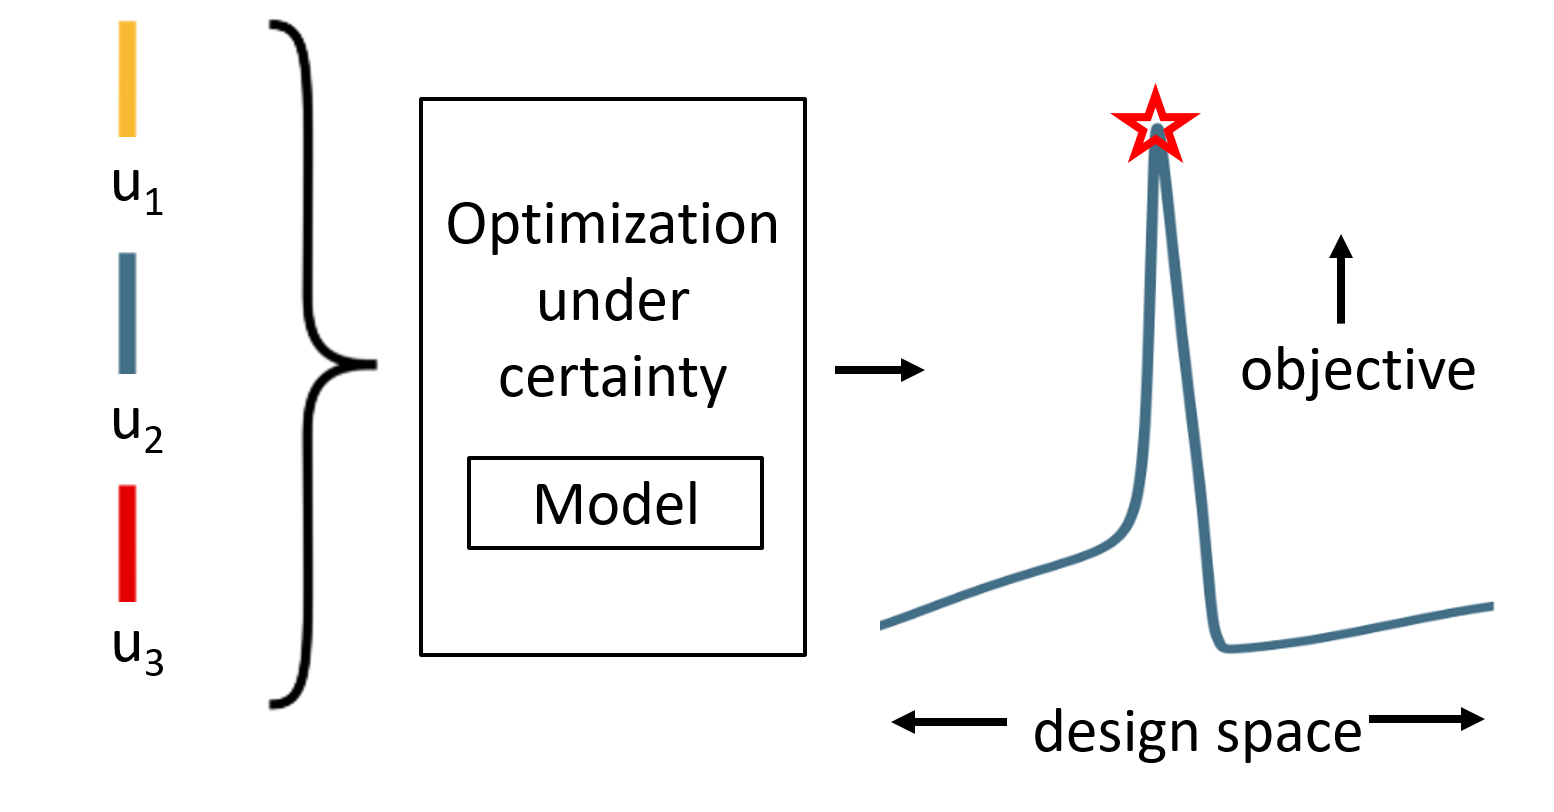
\includegraphics[width=.8\linewidth]{ouc.PNG}
    \end{subfigure}
    \begin{subfigure}{.49\textwidth}
    \centering
        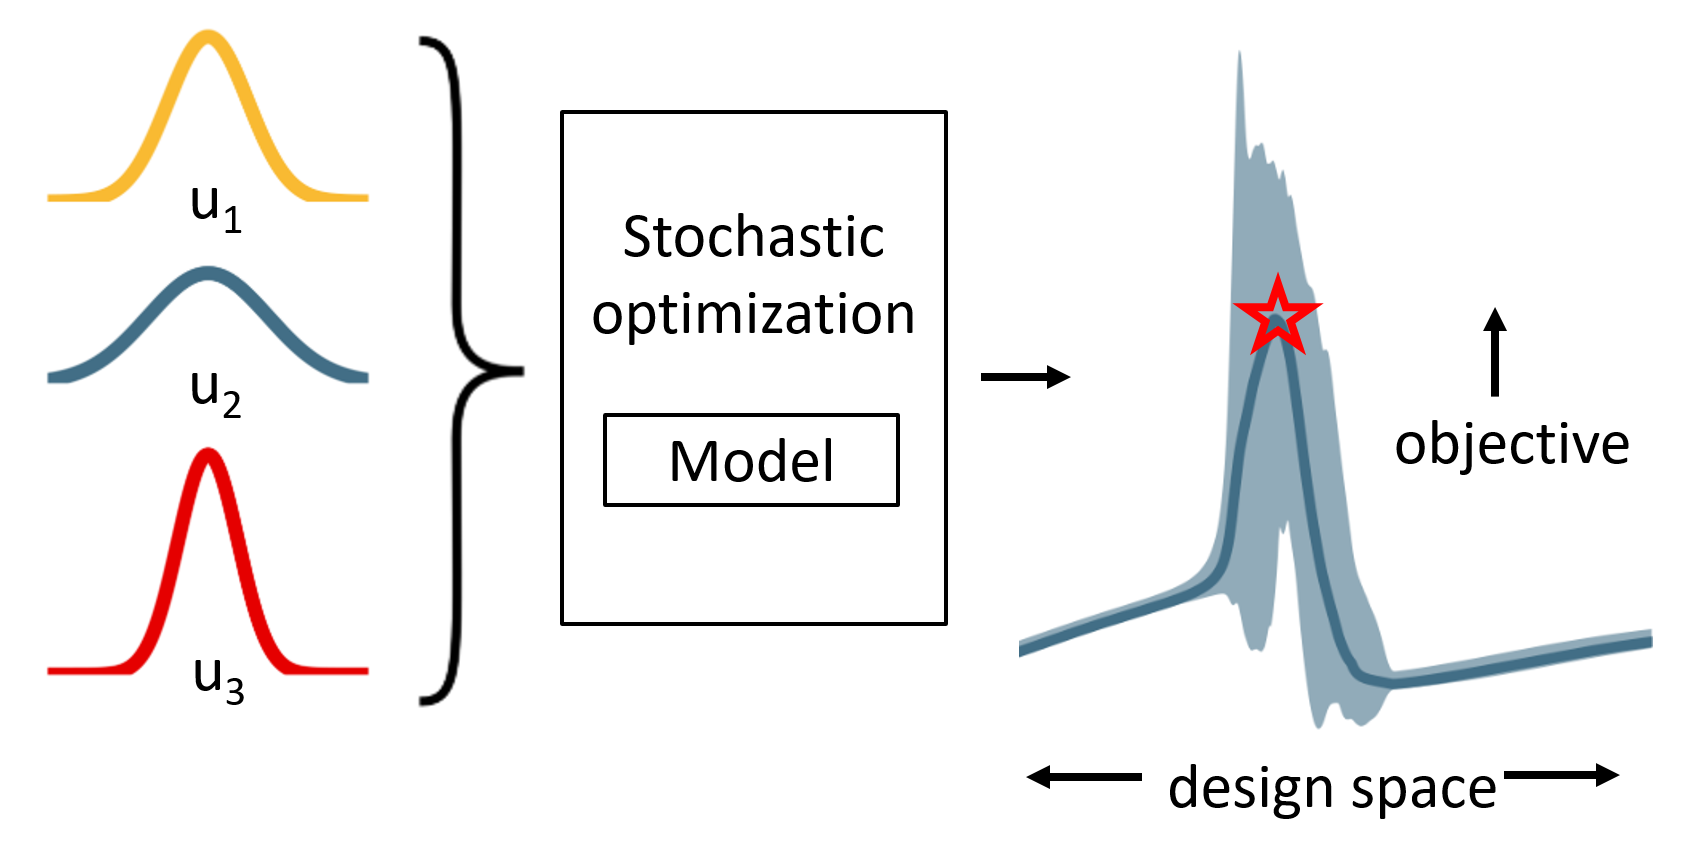
\includegraphics[width=.9\linewidth]{so.PNG}
    \end{subfigure}
    \begin{subfigure}{.49\textwidth}
    \centering
        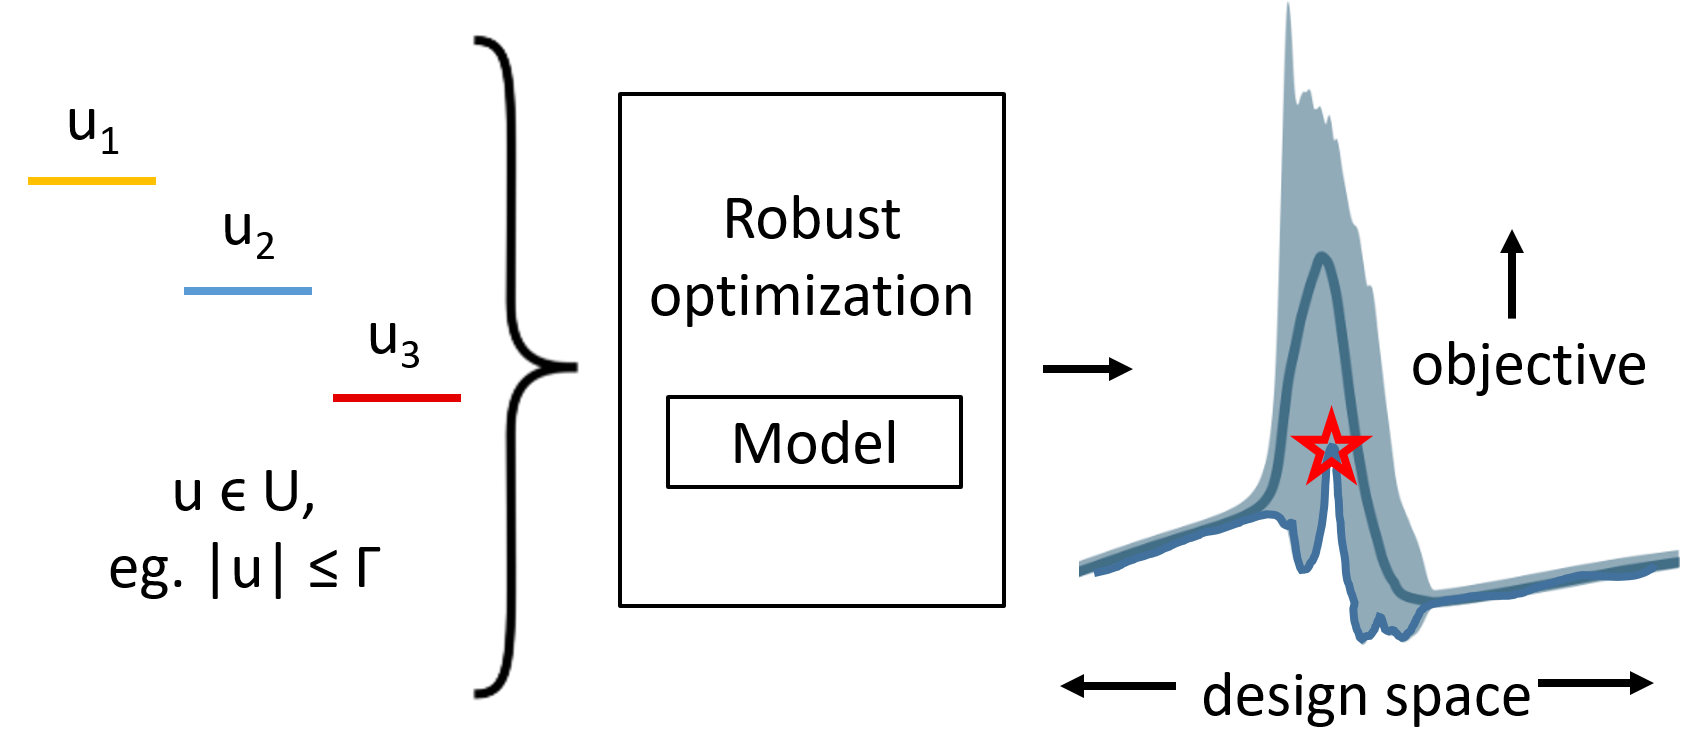
\includegraphics[width=.9\linewidth]{ro.PNG}
    \end{subfigure}
    \caption{\gls{so} and \gls{ro} are methods for optimization under uncertainty that use different definitions
             of uncertain inputs and produce different objective outcomes.}
    \label{fig:approaches}
\end{center}
\end{figure}

{\color{blue}\gls{so} pairs well with gradient-based approaches to solving nonlinear optimization problems
such as those defined in ~\cite{Gallard2013},~\cite{Liem2015} and ~\cite{Liem2017}.
These approaches implement an iterative process where
the objective function and constraints are evaluated over an initial design, and first- and/or
second-order information are used to converge the design towards a local optimum.
In this context, \gls{so} problems deal with uncertainty by including
probability distributions of the uncertain parameters in the iteration, and propagating
the distributions through the physics of a design problem to ensure constraint feasibility with certain probability.
The predominant goal of \gls{so} is to optimize some distributional
characteristics, eg. the mean as in Figure~\ref{fig:approaches},
of the probability density function of the objective~\cite{Diwekar2008}.}

{\color{blue}There have been recent developments in multi-mission aircraft design
using stochastic optimization.
Liem et. al~\cite{Liem2015} propose optimally
weighted objective functions over an aircraft's operational
design envelope for robust aircraft design.
In a follow-up work, Liem et al. generate probability distributions
of uncertain parameters from data
and minimize the expectation of an objective function over
parameter distributions~\cite{Liem2017}.
Although these stochastic methods demonstrate significant improvements over
legacy design methods in terms of design robustness,
they do not address many of the aforementioned challenges of legacy design methods
in capturing the robustness-optimality tradeoff.
The scope of the design problems is narrow and limited to aerostructural optimization,
and the number of uncertain parameters is low.
The formulations assume the presence of data, limiting the
effectiveness of the methods in conceptual design.
They have large computational costs that are somewhat mitigated through
surrogate modeling, but would be detrimental in the conceptual design phase.
Most importantly, they lack rigorous mathematical assessments of design feasibility
under uncertain parameters.}

In contrast to \gls{so},
\gls{ro} can only be applied to mathematical programs that have a robust counterpart,
such as linear, quadratic, semidefinite and geometric programs.
\gls{ro} takes a different approach than \gls{so} in both the form
of uncertain inputs and the objective functions. \gls{ro} produces designs that are
immune to constraint violations as long as parameter values come from within a defined
uncertainty set. The objective of \gls{ro} is to optimize the
the worst-case objective outcome of a design for a
given set over the uncertain parameters. As such,
\gls{ro} avoids the need to sample and propagate probability
distributions, and turns stochastic optimization problems into
deterministic problems that are efficiently solved.}

\subsection{Comparison of robust and stochastic optimization methods for conceptual design}
\label{sec:robustvsstochastic}

Both \gls{ro} and \gls{so} have relative advantages in implementation. This paper will
argue specifically that the formulation of conceptual engineering design problems under uncertainty as
\gls{ro} problems has advantages over \gls{so} formulations (a more
mathematical programming centric comparison is made in~\cite{Bertsimas2011}).

\subsubsection{Generality and tractability}

In the context of engineering, we claim that an optimization method is general
when it can be used to solve a range of problems of interest. On the other hand,
tractability describes whether or not the problems are solved to a satisfactory
optimum within reasonable computational time. Optimization
under uncertainty is a difficult task that puts these two desirable subjective traits
at odds with each other.

\gls{so} has the advantage of generality.
\gls{so} methods are easily applicable to black box models or input-output systems.
They require little knowledge, if any, about the constraints in the system of interest.
\gls{ro} methods are less general, since they require
the design objective and constraints to be explicit and cast in a form that has a worst-case
counterpart. Thus models for \gls{ro} have to be transparent,
and \gls{ro} cannot be applied to black box models without significant prior data
manipulation and fitting at a minimum. A mitigating factor is that
many classes of conceptual engineering design problems can be cast or approximated in a form that
is compatible with robust optimization.

On the other hand, \gls{ro} is more tractable than \gls{so} due to the difference in method of uncertainty propagation.
As aforementioned, \gls{so} methods involve the propagation of probability densities throughout a model
to determine their effects on constraint feasibility and the objective function.
This requires the integration of the product of probability distributions with potential outcomes,
and since the integration of continuous functions is difficult this is often achieved through
a combination of high-dimensional quadrature and discretizations of the uncertainty into
possible scenarios. This propagation method
results in a combinatorial explosion of possible outcomes which need to be evaluated to determine constraint
satisfaction and the distribution of the objective. Few problems can be addressed purely
through stochastic optimization
(eg. recourse problems~\cite{Kall1982},\cite{Higle1991}; energy planning problems~\cite{Pereira1991};
and certain aircraft design problems ~\cite{Liem2015},\cite{Liem2017}), and
even these are limited by combinatorics and costly system evaluations. Furthermore, they require
problem-specific approximations, so that generality is compromised.
Robust versions of tractable optimization problems are not
guaranteed to be tractable, but in practice the aforementioned classes of optimization problems
have tractable robust formulations~\cite{Bertsimas2011}. In \gls{ro},
there are no separate optimization and evaluation
loops by construction, and thus \gls{ro} problems can be solved to optimality
many orders of magnitude faster than \gls{so} problems of the same form~\cite{Bertsimas2011}.

Conceptual design optimization values generality, because engineers would like to
apply methods for optimization under uncertainty without significant mathematical groundwork,
and tractability, because fast solution times are critical
to reduce program risk early on in the design process when more aspects
of the design are fluid. From this perspective, the relative intractability of
\gls{so}-based approaches makes them unreliable for conceptual design, since significant time is
needed both to develop problem-specific tractable formulations, and to find satisfactory optima.
Furthermore,
many engineering design problems such as aircraft design are approximable by optimization
forms that have tractable robust counterparts, making \gls{ro} better suited
to conceptual design.

\subsubsection{Use of data}

\gls{so} problems generally require complete knowledge of the probability distribution of
parameters.
\gls{ro} requires only `modest assumptions  about distributions, such as a known mean and
bounded support'~\cite{Chen2007}. Since \gls{ro} does not require as much information
about uncertain parameters as \gls{so} does, it can better address conceptual design problems where there
is a lack of experience, or sparse and noisy data~\cite{Bertsimas2011}. It is arguable that \gls{ro}
leaves a lot on the table by not taking advantage of distributional information,
however there is a growing body of research on distributionally robust optimization~\cite{Bertsimas2017}
which seeks to leverage existing data.

\subsubsection{Stochasticity and probabilistic guarantees}

Although \gls{ro} problems solve problems with uncertainty,
\gls{ro} formulations result in \emph{deterministic}\footnote{Determinism in this case
refers to the outcomes of free variables in the optimization model.
Different instances of a deterministic design problem with
the same parameters will result in the same solution.} solutions that are immune
to all possible realizations of parameters in an uncertainty set~\cite{Bertsimas2011}.
There is extensive literature on \gls{ro} methods
that offer differing levels of conservativeness~\cite{Bertsimas2004}
depending on the kind of uncertainty set considered, that are guaranteed
to be feasible over the set of interest.

\gls{so} formulations provide no probabilistic guarantees
since the optimum depends on realizations of random variables\cite{Shmoys2004}.
This is not satisfactory from an engineering perspective, since
optimization runs over the same parameters may result in different
solutions. Furthermore, designs
can be sensitive to issues in sampling schemes over potentially unknown
probability distributions. In the context of engineering design, the determinism
and probabilistic guarantees of \gls{ro} makes
it superior to \gls{so}.

It is important to highlight that,
although both \gls{ro} and \gls{so} seek to address the problem
of optimization under uncertainty, they solve fundamentally different problems. In an ideal world where
we have a problem that is tractable and globally optimal for both methods, the two different
approaches would result in different solutions.

\subsection{Geometric and signomial programming for engineering design}

Geometric programming\footnote{Programming refers to the mathematical formulation of an optimization problem.}
is a method of log-convex optimization that has been developed
to solve problems in engineering design~\cite{Duffin1967}. Although theory of the \gls{gp} has existed since
the 1960's, \gls{gp}s have recently experienced a resurgence due to the advent of polynomial-time
interior point methods~\cite{Nesterov1994} and improvements in computing. They have been
applied to a range of engineering design problems with success. For a non-exhaustive list of examples,
please refer to~\cite{Boyd2007}.

\gls{gp}s have been effective in aircraft conceptual design
(\cite{Hoburg2013},~\cite{Burton2017}).
However, the stringent mathematical form of a \gls{gp} means it can only be applied to log-convex problems.
The \gls{sp} is the difference-of-log-convex extension of the \gls{gp} which can be applied to
solve this larger set of problems, albeit with the loss of some mathematical guarantees compared to the \gls{gp}~\cite{Kirschen2018}.
Aircraft pose some of the most challenging design problems~\cite{York2018}, and signomial programming
has been used to great effect in modeling and designing complex aircraft at a conceptual level quickly
and reliably as in \cite{York2018}, \cite{Kirschen2018} and \cite{Kirschen2016}.
Other interesting applications for SPs such as in network flow problems are being investigated.

Robust formulations exist for solving geometric programs with parametric uncertainty~\cite{Saab2018}.
The creation of a robust signomial programming framework to capture uncertainty in engineering
design, and specifically aircraft design, will allow us to have more confidence in the results
of the conceptual design phase, reduce program risk, and increase overall system performance.

\subsection{Contributions}

This paper proposes a tractable \gls{rsp} which we solve as a sequential \gls{rgp},
allowing us to implement robustness in non-log-convex problems such as aircraft design.
We extend the \gls{rgp} framework developed by Saab~\cite{Saab2018} to \gls{sp}s.
We implement the \gls{rsp} formulation on a conceptual aircraft design problem with over a hundred
variables as defined in~\cite{Ozturk2018}.
The benefits of \gls{ro} are demonstrated both in ensuring design feasibility and performance
using \gls{mc} simulations of the uncertain parameters.
We further explore the benefits of \gls{ro} in multiobjective optimization, and propose
a goal programming \gls{rsp} formulation for risk minimization problems.




\section{Mathematical Background}

\subsection{Robust Optimization}

Given a general optimization problem under parametric uncertainty, we define the set of possible
realizations of uncertain vector of parameters $u$ in the uncertainty set $\mathcal{U}$. This
allows us to define the problem under uncertainty below.

\begin{align*}
    \text{min} &~f_0(x) \\
    \text{s.t.}     &~f_i(x,u) \leq 0,~\forall u \in \mathcal{U},~i = 1,\ldots,n \\
\end{align*}

This problem is infinite-dimensional, since it is possible to formulate an infinite number of constraints
with the countably infinite number of possible realizations of $u \in \mathcal{U}$. To circumvent this issue,
we can define the following robust formulation of the uncertain problem below.

\begin{align*}
    \text{min} &~f_0(x) \\
    \text{s.t.}     &~\underset{u \in \mathcal{U}}{\text{max}}~f_i(x,u) \leq 0,~i = 1,\ldots,n \\
\end{align*}

This formulation hedges against the worst-case realization of the uncertainty in the defined uncertainty
set. The set is often described by a norm, which contains possible uncertain outcomes from distributions with
bounded support

\begin{equation}
\begin{aligned}
    \text{min} &~f_0(x) \\
    \text{s.t.}     &~\underset{u}{\text{max}}~f_i(x,u) \leq 0,~i = 1,\ldots,n \\
                    &~\norm{u} \leq \Gamma \\
\end{aligned}
        \label{eq:normform}
\end{equation}

where $\Gamma$ is defined by the user as a global uncertainty bound. The larger the $\Gamma$,
the greater the size of the uncertainty set that is protected against.

\subsection{Geometric Programming}

A \emph{geometric program in posynomial form} is a log-convex optimization problem of the form:

\begin{equation}
\begin{aligned}
	& \text{min} && f_0 \left(\vec{u}\right) \\
	& \text{s.t.} && f_i \left(\vec{u}\right) \leq 1, i = 1,...,m_p\\
	& && h_i \left(\vec{u}\right) = 1, i = 1, ...,m_e\\
\end{aligned}
\label{GP_standard}
\end{equation}
where each $f_i$ is a {\em posynomial}, each $h_i$ is a {\em monomial}, $m_p$ is the number of posynomials,
and $m_e$ is the number of monomials. A monomial $h(\vec{u})$ is a function of the form:

\begin{displaymath}
	h_i(\vec{u}) = e^{b_i}\textstyle{\prod}_{j=1}^{n}{u_j}^{a_{ij}}
\end{displaymath}

where $a_{ij}$ is the $j^{th}$ component of a row vector $\vec{a_i}$ in $\mathbb{R}^n$,
$u_j$ is the $j^{th}$ component of a column vector $\vec{u}$ in $\mathbb{R}^n_+$ ,
and $b_i$ is in $\mathbb{R}$. An example of a monomial is the lift equation,
$L = \frac{1}{2}\rho V^2 C_L S$.
A posynomial $f(\vec{u})$ is the sum of $K \in \mathbb{Z}^+$ monomials:

\begin{displaymath}
	f_i(\vec{u}) = \textstyle{\sum_{k=1}^{K}}e^{b_{ikj}}\prod_{j=1}^{n}{u_j}^{a_{ikj}}
\end{displaymath}

where $a_{ikj}$ is the $j^{th}$ component of a row vector $\vec{a_{ik}}$ in $\mathbb{R}^n$,
$u_j$ is the $j^{th}$ component of a column vector $\vec{u}$ in $\mathbb{R}^n_+$, and $b_{ik}$
is in $\mathbb{R}$ \cite{Boyd2007}. The stagnation pressure definition is a good example:
$P_t = P + \frac{1}{2} \rho V^2$.\\

A logarithmic change of the variables $x_j = \log(u_j)$ would turn a monomial into
{\em  the exponential of an affine function} and a posynomial into
{\em the sum of exponentials of affine functions}. A transformed monomial $h_i(\vec{x})$ is a function of the form:

\begin{displaymath}
    h_i(\vec{x}) = e^{\vec{a_i}\vec{x} + b_i}
\end{displaymath}

where $\vec{x}$ is a column vector in $\mathbb{R}^n$.
A transformed posynomial $f_i(\vec{x})$ is the sum of $K_i \in \mathbb{Z}^+$ monomials:

\begin{displaymath}
    f_i(\vec{x}) = \textstyle{\sum_{k=1}^{K_i}}e^{\vec{a_{ik}}\vec{x} + b_{ik}}
\end{displaymath}

where $\vec{x}$ is a column vector in $\mathbb{R}^n$.
A geometric program with transformed constraints is a \emph{geometric program in exponential form}, and
is a convex optimization problem.

The positivity of exponential functions restricts the space spanned by posynomials and limits
\gls{gp}s to certain classes of problems.
However, since many engineering problems of interest have purely positive quantities \gls{gp}s
are quite applicable, and certain variable transformations can make problems with negative quantities tractable.
The restriction of posynomials to the \emph{less-than-side of
inequalities} is a more significant barrier, and motivates the introduction of signomials.

\subsection{Signomial Programming}
A {\em signomial} can be defined as the difference between two posynomials. Consequently,
a \gls{sp} is a non-log-convex optimization problem of the form:

\begin{equation}
\begin{aligned}
&\text{minimize } && f_{0}(\vec{x}) \\
&\text{subject to } && f_{i}(\vec{x}) - g_{i}(\vec{x})& \leq 0, i = 1, ...., m \\
\end{aligned}
\end{equation}

where $f_{i}$ and $g_{i}$ are both posynomials, and $\vec{x}$ is a column vector in $\mathbb{R}^n$. 

Reliably solving an \gls{sp} to a local optimum has been described in \cite{Boyd2007} and \cite{Lipp2016}.
A common solution heuristic involves solving an \gls{sp} as a sequence of \gls{gp}s,
where each \gls{gp} is a local approximation of the \gls{sp}.
Although it is a powerful tool, applications involving \gls{sp}s are usually prone
to uncertainties that have a significant effect on the solution.


\section{Robust Signomial Programming} \label{RSP}
Robust signomial programming assumes that parameter uncertainties belong to an uncertainty set, and solves the design problem to find the best solution
as shown in Figure~\ref{fig:blockdiag}. This section introduces gls{rsp}s and derives the intractable formulation of an gls{rsp}.

%\begin{figure}[h]
%	\centering
%	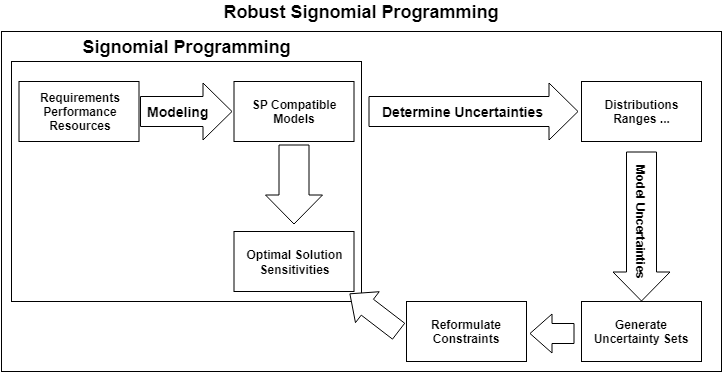
\includegraphics{figures/RSP_Diagram.png}
%	\caption{A block diagram showing the difference between the design process using an SP and an RSP.}
%	\label{block_diag}
%\end{figure}

\begin{figure}
    \begin{center}
    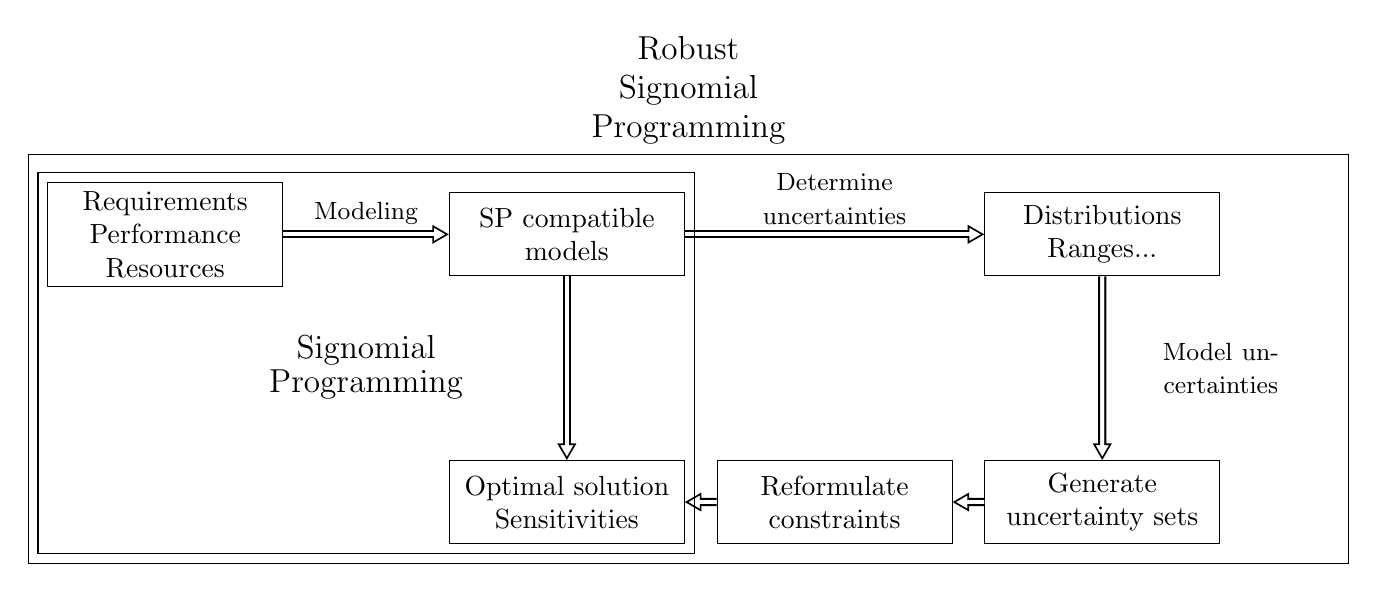
\begin{tikzpicture}[auto, align=center, text width=2.75cm, scale = 0.85]
        \begin{scope}[node distance=2cm]
        \node[block, name=reqs] at (0,0) (reqs) {Requirements \\ Performance \\ Resources};
        \node[block, name=SPmodels] at (6,0) (SPmodels) {SP compatible \\ models};
        \node[block, name=optimum] at (6,-4) (optimum) {Optimal solution \\ Sensitivities};
        \node[block, name=distr] at (14,0) (distr) {Distributions \\ Ranges...};
        \node[block, name=sets] at (14,-4) (sets) {Generate \\ uncertainty sets};
        \node[block, name=reformulate] at (10,-4) (reformulate) {Reformulate constraints};
		\node[name=dummy] at (6, 0.5) (dummy) {};

		    \draw[vecArrow] (reqs) -- node[name=modeling] {\small Modeling} (SPmodels);
			\draw[vecArrow] (SPmodels)to (optimum);
			\draw[vecArrow] (SPmodels) -- node[name=detuncert] {\small Determine uncertainties} (distr);
			\draw[vecArrow] (distr) -- node[name=modeluncert] {\small Model uncertainties} (sets);
 			\draw[vecArrow] (sets) to (reformulate);
			\draw[vecArrow] (reformulate) to (optimum);

		\node[name=SP,label={[xshift=0.0cm, yshift=-3.0cm]\large Signomial Programming},fit=(reqs)(SPmodels)(optimum), draw] {};
		\node[name=RSP,label={[xshift=0.0cm, yshift=0.0cm]\large Robust \\ Signomial \\ Programming \\},
		fit=(SP)(reqs)(SPmodels)(optimum)(distr)(sets)(reformulate)(modeluncert)(detuncert)(modeling)(dummy), draw] {};
		\end{scope}
    \end{tikzpicture}
    \caption{A block diagram showing the difference between the design process using an \gls{sp} and an \gls{rsp}.}
        \label{fig:blockdiag}
\end{center}
\end{figure}


An SP in its \textbf{exponential form} is as follows:

\begin{equation}
    \label{SP_exponential}
\begin{aligned}
	& \min && f_0\left(\vec{x}\right) \\
	& \text{s.t.} && \textstyle{\sum}_{k=1}^{K_i}e^{\vec{a_{ik}}\vec{x} + b_{ik}} - \textstyle{\sum}_{k=1}^{G_i}e^{\vec{c_{ik}}\vec{x} + d_{ik}} \leq 0 \quad \forall i \in 1,...,m\\
\end{aligned}
\end{equation}

Let $\vec{a_{ik}}$ and $\vec{c_{ik}}$ be the $((i-1)\times m + k)^{th}$ rows of the exponents matrices $\mat{A}$ and $\mat{C}$ respectively, and $b_{ik}$ and $d_{ik}$ be the $((i-1)\times m + k)^{th}$ elements of the coefficients vectors $\vec{b}$ and $\vec{d}$ respectively.

The data ($\mat{A}$, $\mat{C}$, $\vec{b}$, $\vec{d}$) is assumed uncertain and living in an uncertainty set $\mathcal{U}$, where $\mathcal{U}$ is parametrized affinely by a perturbation vector $\vec{\zeta}$ as follows:

\begin{equation}
\mathcal{U} = \left\{\left[\mat{A};\mat{C};\vec{b};\vec{d}\right] = \left[\mat{A}^0;\mat{C}^0;\vec{b}^0\;\vec{d}^0 \right] + \textstyle{\sum_{l=1}^{L}\zeta_l\left[\mat{A}^l;\mat{C}^l;\vec{b}^l; \vec{d}^l\right]}\right\}
\label{Data}
\end{equation}
where $\mat{A}^0$, $\mat{C}^0$, $\vec{b}^0$, and $\vec{d}^0$ are the nominal exponents and coefficients, $\left\{\mat{A}^l\right\}_{l=1}^{L}$, $\left\{\mat{C}^l\right\}_{l=1}^{L}$, $\left\{\vec{b}^l\right\}_{l=1}^{L}$, and $\left\{\vec{d}^l\right\}_{l=1}^{L}$ are the basic shifts of the exponents and coefficients, and $\zeta_l$ is the $l^{th}$ component of $\vec{\zeta}$ belonging to a perturbation set $\mathcal{Z} \in \mathbb{R}^L$ such that
\begin{equation}
\mathcal{Z} = \left\{ \vec{\zeta} \in \mathbb{R}^L: \norm{\vec{\zeta}} \leq \Gamma \right\}
\label{perturbation_set}
\end{equation}

As mentioned earlier, there should exist a formulation immune to
uncertainty in the system's data. Accordingly, the robust counterpart
of the uncertain \gls{sp} in \eqref{SP_exponential} is:

\begin{equation}
\begin{aligned}
& \min &&f_0\left(\vec{x}\right)\\
& \text{subject to} &&\max_{\vec{\zeta} \in \mathcal{Z}} \left\{\textstyle{\sum}_{k=1}^{K_i}e^{\vec{a_{ik}}\left(\zeta\right)\vec{x} + b_{ik}\left(\zeta\right)} - \textstyle{\sum}_{k=1}^{G_i}e^{\vec{c_{ik}}\left(\zeta\right)\vec{x} + d_{ik}\left(\zeta\right)}\right\} &&\leq 1 &&\forall i \in 1,...,m\\
\end{aligned}
\label{SP_counterparts_finite}
\end{equation}

The optimization problem in \eqref{SP_counterparts_finite} is intractable using current solvers,
therefore,  a heuristic approach to solving \gls{rsp}s approximately
as a sequential RGP will be presented in the following sections.
As our approach is based on Robust Geometric Programming, a brief review of the subject will follow based on \cite{Saab2018}.


\section{Robust Geometric Programming} \label{RGP}

This section presents a brief review of the approximation of an RGP as a
tractable optimization problem as discussed in~\cite{Saab2018}.
The robust counterpart of an uncertain geometric program is:
\begin{equation}
\begin{aligned}
& \min &&f_0\left(\vec{x}\right)\\
& \text{subject to} &&\max_{\vec{\zeta} \in \mathcal{Z}} \left\{\textstyle{\sum}_{k=1}^{K_i}e^{\vec{a_{ik}}\left(\zeta\right)\vec{x} + b_{ik}\left(\zeta\right)}\right\} &&\leq 1 &&\forall i \in 1,...,m\\
\end{aligned}
\label{GP_counterparts_finite}
\end{equation}
which is Co-NP hard in its natural posynomial form \cite{RGPcoNP}. We will present three approximate formulations of a \gls{rgp}.

\subsection{Simple Conservative Formulation}
One way to approach the intractability in \eqref{GP_counterparts_finite} is to replace each constraint by a tractable approximation.
Replacing the max-of-sum in \eqref{GP_counterparts_finite} by the sum-of-max will lead to the following formulation.
\begin{equation}
\begin{aligned}
& \min &&f_0\left(\vec{x}\right)\\
& \text{subject to} &&\textstyle{\sum}_{k=1}^{K_i} {\displaystyle \max_{\vec{\zeta} \in \mathcal{Z}}} \left\{e^{\vec{a_{ik}}\left(\zeta\right)\vec{x} + b_{ik}\left(\zeta\right)}\right\} &&\leq 1 &&\forall i \in 1,...,m
\end{aligned}
\label{GP_safe_conservative}
\end{equation}
Maximizing a monomial term is equivalent to maximizing an affine function, therefore \eqref{GP_safe_conservative} is tractable.

\subsection{Equivalent Intermediate Formulation}

This formulation is equivalent to the formulation in \eqref{GP_counterparts_finite}, but with smaller, easier to handle posynomial constraints.
By the properties of inequalities, the posynomial $P$ in posynomial inequality $ M \geq  P$ can be
divided into an equivalent set of smaller posynomials based on the dependence between its monomial terms.
Figure~\ref{fig:partitioning} shows how a constraint can be represented as an equivalent set of smaller posynomial constraints.

\begin{figure}
    \begin{center}
        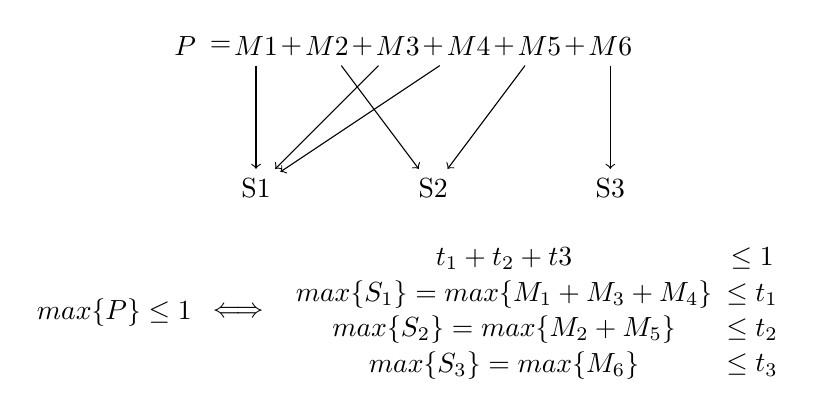
\begin{tikzpicture}[auto,scale = 0.9]
            \begin{scope}[node distance=0.5cm]
                \node[name=P] at (0,0) (P) {$P$};
                \node[name=equals] at (0.5,0) (equals) {$=$};
                \node[name=M1] at (1,0) (M1) {$M1$};
                \node[name=M2] at (2,0) (M2) {$M2$};
                \node[name=M3] at (3,0) (M3) {$M3$};
                \node[name=M4] at (4,0) (M4) {$M4$};
                \node[name=M5] at (5,0) (M5) {$M5$};
                \node[name=M6] at (6,0) (M6) {$M6$};
                \node[name=p1] at (1.5,0) (p1) {$+$};
                \node[name=p2] at (2.5,0) (p2) {$+$};
                \node[name=p3] at (3.5,0) (p3) {$+$};
                \node[name=p4] at (4.5,0) (p4) {$+$};
                \node[name=p5] at (5.5,0) (p5) {$+$};
                \node[name=S1] at (1,-2) (S1) {S1};
                \node[name=S2] at (3.5,-2) (S2) {S2};
                \node[name=S3] at (6,-2) (S3) {S3};
                \draw[->] (M1) -- (S1);
                \draw[->] (M3) -- (S1);
                \draw[->] (M4) -- (S1);
                \draw[->] (M2) -- (S2);
                \draw[->] (M5) -- (S2);
                \draw[->] (M6) -- (S3);
                \node[name=t1, align=left] at (8, -3) (t1) {$\leq 1$};
                \node[name=t2, align=left] at (8, -3.5) (t1) {$\leq t_1$};
                \node[name=t3, align=left] at (8, -4) (t1) {$\leq t_2$};
                \node[name=t4, align=left] at (8, -4.5) (t1) {$\leq t_3$};
                \node[name=arrow] at (0.75,-3.75) (arrow) {$\Longleftrightarrow$};
                \node[name=orig] at (-1,-3.75) (orig) {$max\{P\} \leq 1$};
                \node[name=c1, align=left] at (4.5,-3) (c1) {$t_1 + t_2 + t3$};
                \node[name=c2, align=left] at (4.5,-3.5) (c2) {$max\{S_1\} = max\{M_1 + M_3 + M_4\}$};
                \node[name=c3, align=left] at (4.5,-4) (c3) {$max\{S_2\} = max\{M_2 + M_5\}$};
                \node[name=c4, align=left] at (4.5,-4.5) (c4) {$max\{S_3\} = max\{M_6\}$};

            \end{scope}
        \end{tikzpicture}
        \caption{Partitioning of a large posynomial into smaller posynomials requires the addition of auxiliary variables. $S_i$
        are posynomials with independent sets of variables.}
        \label{fig:partitioning}
    \end{center}
\end{figure}

The posynomial constraints are categorized into three sets: large posynomials, two-term posynomials and monomials,
represented by $S1$, $S2$ and $S3$ respectively.
Monomials are tractable, and two-term posynomials can be well approximated using piecewise-linear
functions~\cite{hsiung_kim_boyd_2007}.
We implement the following two tractable approximations for large posynomials.

\subsubsection{Linearized Perturbations Formulation}
If the exponents are known and certain, then large posynomial constraints can be approximated as signomial constraints.
The exponential perturbations in each posynomial are linearized using a modified least squares method, and then the
posynomial is robustified using techniques from robust linear programming. The resulting set of constraints is \gls{sp} compatible,
therefore, a \gls{rgp} can be approximated as a \gls{sp}.

\subsubsection{Best Pairs Formulation}
If the exponents are also uncertain, then large posynomials can't be approximated as an \gls{sp}, and further simplification is needed.
This formulation aims to maximize each pair of monomials in each posynomial,
while finding the best combination of monomials that gives the least conservative solution.
\cite{Saab2018} provides a descent algorithm to find locally optimal combinations of the monomials,
and shows how the uncertain \gls{gp} can be approximated as a \gls{gp} for polyhedral uncertainty,
and a conic optimization problem for elliptical uncertainty with uncertain exponents.
For a detailed description of the above formulations refer to \cite{Saab2018}.
An algorithm for solving an \gls{rsp} based on the above formulations is provided in the next section.


\section{Approach to Solving Robust Signomial Programs}

This section presents a heuristic algorithm to solve a \gls{rsp}
based on our previous discussion on robust geometric programming.

\subsection{General \gls{rsp} Solver}
As mentioned before, a common heuristic algorithm to solve a \gls{sp} is
by sequentially solving local \gls{gp} approximations, but the solution is not guaranteed
to be globally optimal. Our approach to solve a \gls{rsp} is based on sequentially solving
local \gls{rgp} approximations. Below we provide a step-by-step algorithm to solve a \gls{rsp}:

\begin{enumerate}
    \item Choose an initial guess $x_0$.
    \item Repeat:
    \begin{enumerate}
        \item Find the local GP approximation of the \gls{sp} at $x_i$.
        \item Find the RGP formulation of the GP.
        \item Solve the RGP to obtain $x_{i+1}$.
        \item If $x_{i+1} \approx x_{i}$: break
    \end{enumerate}
\end{enumerate}

Similar to a \gls{sp}, a good initial guess will lead to faster convergence and possibly a better solution.
The deterministic solution of the uncertain \gls{sp} is a good candidate $x_0$,
and is used to speed up convergence.

\begin{figure}
    \begin{center}
    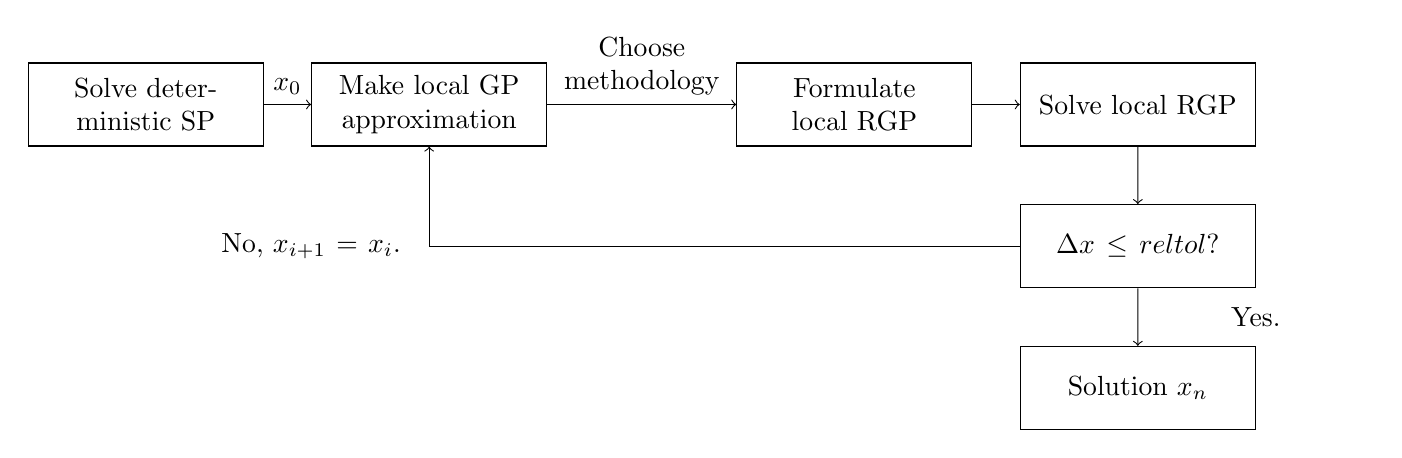
\begin{tikzpicture}[auto, align=center, text width=2.75cm, scale = 0.9]
        \begin{scope}[node distance=2cm]
        \node[block, name=detSP] at (0,0) (detSP) {Solve deterministic SP};
        \node[block, name=localGP] at (4,0) (localGP) {Make local GP approximation};
        \node[block, name=localRGP] at (10,0) (localRGP) {Formulate local RGP};
        \node[block, name=solveRGP] at (14,0) (solveRGP) {Solve local RGP};
        \node[block, name=xi] at (14,-2) (xi) {$\Delta x \leq reltol$?};
        \node[block, name=solution] at (14,-4) (solution) {Solution $x_{n}$};

        \draw[->] (detSP) -- node[name=x0] {$x_0$} (localGP);
        \draw[->] (localGP) -- node[name=choosemethod] {Choose methodology} (localRGP);
        \draw[->] (localRGP) -- (solveRGP);
        \draw[->] (solveRGP) -- (xi);
        \draw[->] (xi) -| node[name=no] {No, $x_{i+1} = x_i.$} (localGP);
        \draw[->] (xi) -- node[name=yes] {Yes.} (solution);
        \end{scope}
    \end{tikzpicture}
    \caption{A block diagram showing the steps of solving an \gls{rsp}.}
        \label{fig:rspsolve}
\end{center}
\end{figure}

Any of the previously mentioned methodologies can be used to formulate the local RGP approximation. 
However, depending on the RGP formulation chosen to solve a \gls{rsp}, the last formulation and solution
blocks in Figure \ref{fig:rspsolve} are adjusted for a faster rate of convergence.
\ \\
\subsection{Best Pairs \gls{rsp} Solver}

If the Best Pairs methodology is exploited, then the above algorithm would change so that
each iteration would solve the local RGP approximation and choose the best permutation
for each large posynomial. The modified algorithm would become as follows:

\begin{enumerate}
    \item Choose an initial guess $x_0$.
    \item Repeat:
    \begin{enumerate}
        \item Find the local GP approximation of the SP at $x_i$.
        \item For each large posynomial constraint, select the new permutation $\phi$
                such that $\phi$ minimizes the robust large constraint evaluated at $x_i$.
        \item Solve the approximate tractable counterparts of the local \gls{gp} in
                \eqref{GP_counterparts_finite}, and let $\vec{x}_{i+1}$ be the solution.
        \item If $x_{i+1} \approx x_{i}$: break.
    \end{enumerate}
\end{enumerate}

\subsection{Linearized Perturbations \gls{rsp} Solver}

On the other hand, if the Linearized Perturbations formulation is to be used,
then we can avoid solving a \gls{sp} at each iteration by first
approximating the original \gls{sp} constraints locally, and in the same loop approximating
the robustified possibly signomial constraints locally, thus solving a
\gls{gp} at each iteration instead of an \gls{sp}. The algorithm would then become as follows:

\begin{enumerate}
    \item Choose an initial guess $x_0$.
    \item Repeat:
    \begin{enumerate}
        \item Find the local GP approximation of the SP at $x_i$.
        \item Robustify the constraints of the local GP approximation using the Linearized Perturbations methodology.
        \item Find the local GP approximation of the resulting local SP at $x_i$.
        \item Solve the local GP approximation in step c to obtain $x_{i+1}$.
        \item If $x_{i+1} \approx x_{i}$: break.
    \end{enumerate}
\end{enumerate}


\section{Models}

We implement the \gls{rsp} formulation above on an unmanned, gas-powered
aircraft design problem that is systematically developed in~\cite{Ozturk2018},
with the elliptical fuselage model borrowed from ~\cite{Burton2017}.
We optimize a wing, fuselage, and engine given a payload and range requirement.
The optimization model was developed using GPkit, a Python package that
provides abstractions for using \gls{gp}s in engineering design~\cite{gpkit}.
The nominal model has 176 variables and 154 constraints, a common level of
sparsity for~\gls{gp} and~\gls{sp} models.
A short qualitative overview of the model follows; for
more detailed information, please refer to~\cite{Ozturk2018} and~\cite{Burton2017}. The uncertainties
associated with the parameters will be described in Section~\ref{uncertainties_and_sets}.

\subsection{Flight Profile}

The flight profile models is borrowed from ~\cite{York2018}. Within the model, the
trajectory of the aircraft is optimized over five steady flight segments,
although we are restricted to modeling only climb segments
and therefore the stored gravitational potential energy of the aircraft is not captured.

\subsection{Atmosphere}

The atmosphere model is taken from~\cite{Tao2018}, and considers changes in density and dynamic
viscosity with altitude, for a standard atmosphere.

\subsection{Aircraft}

The aircraft is modeled as a wing, fuselage and engine system. The aircraft is assumed
to be in steady flight, so that the thrust power is equal to the sum of the drag power and rate of change
of potential energy of the aircraft, and the lift is equal to the total weight, ignoring the vertical component of
thrust in climb. Its total weight is the sum of its components.
The aircraft has to be able to takeoff at specified minimum speed without stalling as well.
Aircraft component models are detailed below.

\subsubsection{Wing}

Lift is generated by the wing as a function of its geometry and freestream conditions.
The wing structure model is based on a simple beam model with a distributed lift load,
and a point mass in the center representing the fuselage.
Wing fuel volume is modeled as a fraction of the internal volume available in the wing.
Its drag is
approximated simply as a sum of the induced and profile drags, the latter of which is estimated using a
form factor. The weight of the wing is the sum of skin and spar weights.

\subsubsection{Fuselage}

The fuselage is assumed to be ellipsoidal in shape and to contain fuel and payload.
The fuselage drag is estimated using a form factor.
The fuselage is assumed not to contain any structural members, and so its weight consists only of skin weight.

\subsubsection{Engine}

The aircraft is powered by a naturally aspirated piston engine. It is subject to
power lapse at lower air densities at higher altitudes. Engine weight is modeled using a posynomial fit of existing
engines. \gls{bsfc} is modeled as a function of maximum thrust at a given altitude.

\subsection{Source of non-log-convexity: fuel volume}
The fuel models have been detailed in the previous sections, but it is noteworthy that
the signomial constraint in the optimization appears in the aircraft total fuel volume constraint,
as shown in Equation~\ref{eq:fuel}:

\begin{equation}
\label{eq:fuel}
V_f \leq V_{f_{wing}} + V_{f_{fuse}} 
\end{equation}

The signomial constraints makes the problem non-log-convex, which means that the solution methods
detailed by Saab~\cite{Saab2018} need to be extended to accommodate this optimization problem.


\section{Uncertainties and Sets}
\label{uncertainties_and_sets}

The uncertainties for the different parameters in the problem have been determined
considering the parameters in aircraft design that often have the largest uncertainty.
These uncertainties, given by three times the \gls{cv}\footnote{The \gls{cv}
is defined as follows: $\text{CV} = \frac{\sigma}{|\mu|}$, where $\sigma$ is the standard deviation and $\mu$ is the mean of the parameter.},
are listed in Table~\ref{tab:uncertainties}. Since for the rest of this work
all standard deviations ($\sigma$) are normalized by the means of the parameters, we will use $3\sigma$
to represent $3\text{CV}$.

\begin{table}
\begin{center}
\caption{\label{tab:uncertainties} Parameters and Uncertainties (increasing order)}
\begin{tabular}{c c c c c}
\hline
Parameters & Description & Value & Units &\% Uncert. ($3\sigma$) \\
\hline
$S_{wetratio}$ & wetted area ratio & 2.075 & - & 3\\
e & span efficiency & 0.92 & - & 3\\
$\mu$ & viscosity of air & $1.78 \times 10^{-5}$ & $kg/(ms)$ & 4 \\
$\rho$ & air density & 1.23 & $kg/m^3$ & 5 \\
$C_{L_{max}}$ & stall lift coefficient & 1.6 & - & 5\\
k & fuselage form factor & 1.17 & - & 10\\
$\tau$ & airfoil thickness ratio & 0.12 & - & 10\\
$N_{ult}$ & ultimate load factor & 3.3 & - & 15\\
$V_{min}$ & takeoff speed & 25 & $m/s$ & 20\\
$W_0$ & payload weight & 6250 & $N$ & 20\\
$W_{w_{coeff,i}}$ & wing weight coefficient 1 & $2 \times 10^{-5}$ & $1/m$ & 20\\
$W_{w_{coeff,ii}}$ & wing weight coefficient 2 & 60 & $N/m^2$ & 20\\
\hline
\end{tabular}
\end{center}
\end{table}

The parameter uncertainties reflect aerospace engineering intuition.
The wing weight coefficients $W_{w_{coeff,i}}$ and $W_{w_{coeff,ii}}$, and the ultimate load factor $N_{ult}$ have
large $3\sigma$s because the build quality of aircraft components is
often difficult to quantify with a large degree of certainty.
The payload weight ($W_0$) has a large uncertainty for similar reasons,
since it is often developed concurrently with the aircraft.
Parameters that engineers take to be
physical constants ($\mu$, $\rho$) and those that can be determined or manufactured with a relatively
high degree of accuracy ($S_{wetratio}$, $e$) have relatively low deviations.
Parameters that require testing to determine ($C_{L_{max}}$, $V_{min}$) have a level of uncertainty
that reflects the expected variance of empirical studies. However, note that
these quantities are ultimately picked by the designer and the level of conservatism in the
design will be greatly affected by the chosen $3\sigma$s.


\section{Results}

We implement our \gls{rsp} heuristic algorithm on the aforementioned conceptual aircraft design problem.
Our nominal objective function is total fuel consumption, which is
to be minimized given a payload and a range requirement.

\subsection{Mitigation of probability of failure}

The problem is solved for different sizes of box and elliptical uncertainty sets
by varying the parameter $\Gamma$, as defined in Appendix \ref{LP_to_GP}. Mathematically, for box uncertainty,
$\Gamma$ is a measure of the centered width in logspace of the defined parameter uncertainty, normalized by the
standard deviation of the parameter. For elliptical uncertainty, it is the maximum diameter of the Euclidian norm
ball of $u_i$, which is the number of standard deviations of perturbation of each ith parameter from its nominal value.
Intuitively, it is a measure of how much risk is being hedged against. $\Gamma = 0$
implies that all of the parameters take their nominal values with zero uncertainty,
and larger $\Gamma$ protects against more parameter uncertainty, where a box uncertainty is
more conservative than elliptical uncertainty.

The design variables are then fixed for each solution so that the design can be simulated for
different realizations of the uncertain parameters in Table~\ref{tab:uncertainties}
to examine average design performance. In this~\gls{mc} scheme, the random variables
are simulated from independent and identically distributed $3\sigma$ truncated Gaussians.
We simulate from the truncated Gaussian since this makes it possible to
confirm mathematically that for $\Gamma = 1$, all simulations of uncertain parameters are feasible.
Designs for each solution in Figure~\ref{fig:probOfFailure} are simulated with the same set
of uncertainty realizations for consistency. \\

\begin{figure}[ht]
    \centering
    \captionsetup{justification=centering, font=small}
    \begin{subfigure}{0.49\textwidth}
        \centering
        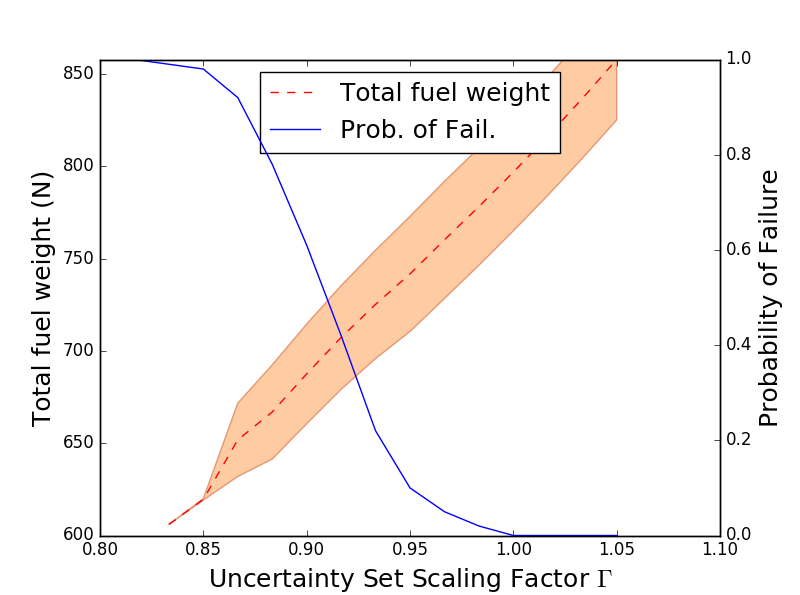
\includegraphics[height=2.3in]{signomial_simple_flight/box_best_pairs.png}
         \caption{Box Uncertainty Set}
    \end{subfigure}%
    ~ 
    \begin{subfigure}{0.49\textwidth}
        \centering
        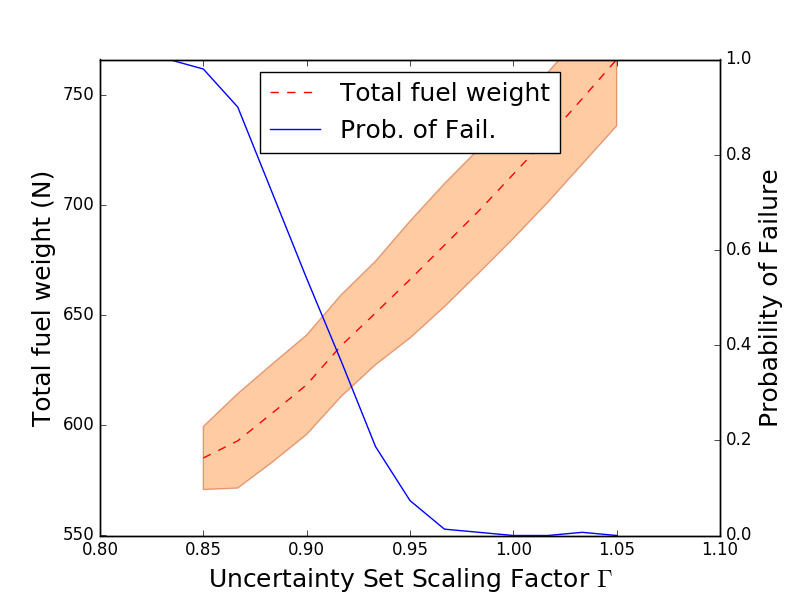
\includegraphics[height=2.3in]{signomial_simple_flight/ell_best_pairs.png}
         \caption{Elliptical Uncertainty Set}
    \end{subfigure}
    \caption{Simulated performance of the optimal robust aircraft, using the Best Pairs formulation,
    as a function of $\Gamma$ for different uncertainty sets.
    The dashed line and the band represent the mean and standard deviation of the performance
    of aircraft designed for different $\Gamma$,
    and simulated with 100 \gls{mc} samples of uncertain parameters.}
    \label{fig:probOfFailure}
\end{figure}

We define the probability of failure of a design as the probability that any constraint
in the design optimization problem is violated in a \gls{mc} simulation.
As expected, Figure \ref{fig:probOfFailure} shows that probability of failure goes to zero as $\Gamma$ increases.
It is noteworthy that, for the nominal problem ($\Gamma = 0$) and for uncertainty up to $\Gamma \leq 0.8$, none of
the 100 simulated uncertain parameters result in feasible solutions. Under uncertain parameters,
the aircraft designed for the average case would almost surely fail to complete its mission.
That being said, it is necessary to sacrifice performance to achieve a high degree ($3\sigma$) of
reliability as in the solution for $\Gamma = 1$.

\begin{table}[!h]
\begin{center}
\caption{\label{tab:results} SP Aircraft Optimization Results}
\begin{tabular}{c c c c c}
\hline
Free variable & Units & No Uncert. & Box [$\Gamma = 1.0$] & Elliptical [$\Gamma = 1.0$] \\
\hline
$L/D$ & - & 40.3 & 31.2 & 34.0 \\
$AR$ & - & 22.6 & 11.8 & 14.5 \\
$Re$ & - & $1.80 \times 10^6$ & $3.59 \times 10^7$ & $3.00 \times 10^6$ \\
$S$ & $\mathrm{m^2}$ & 18.1 & 40.2 & 37.4 \\
$V$ & $\mathrm{m/s}$ & 41.5 & 40.3 & 38.8 \\
$T_{flight}$ & $\mathrm{hr}$ & 20.6 & 21.3 & 22.1 \\
$W_w$ & $\mathrm{N}$ & 2960 & 5060 & 4830 \\
$W_{w,strc}$ & $\mathrm{N}$ & 1880 & 2410 & 2360 \\
$W_{w,surf}$ & $\mathrm{N}$ & 1080 & 2650 & 2470 \\
$V_{f,avail}$ & $\mathrm{m^3}$ & 0.063 & 0.111 & 0.100 \\
$V_{f,fuse}$ & $\mathrm{m^3}$ & 0.005 & 0 & 0 \\
$V_{f,wing}$ & $\mathrm{m^3}$ & 0.058 & 0.111 & 0.100 \\
\hline
E[Objective] & Units & No Uncert. & Box [$\Gamma = 1.0$] & Elliptical [$\Gamma = 1.0$] \\
\hline
$W_{fuel}$ & $\mathrm{N}$ & 502 & 893 & 803 \\
\hline
P[failure] & & No Uncert. & Box [$\Gamma = 1.0$] & Elliptical [$\Gamma = 1.0$] \\
\hline
\% & & 100 & 0 & 0\\
\hline
\end{tabular}
\end{center}
\end{table}

% TODO: update diagrams and graphs with solutions for the problem with composite objective

Moreover, using margins would in the best case be as good as using a box uncertainty set, and therefore will lead
to a more conservative solution with inferior performance.

Figure~\ref{compare_signomial} compares the different methodologies in terms of setup and
run times. Since the setup time of the nominal problem is minimal, we have
normalized the results by the run time of the nominal problem for comparison.
The bottom axis ranks the methods by their level of conservativeness (Best Pairs
and Simple Conservative formulations being the least and most conservative respectively),
and the elliptical formulations are less conservative than the box formulations~\cite{Saab2018}.
For the box uncertainty, solution times increase for increasing levels of conservativeness,
whereas for the elliptical uncertainty they decrease.
%The Best Pairs and Linearized Perturbations methods achieve good performance,
%however the Best Pairs methodology needs the most number of constraints,
%while the Linearized perturbations requires the most setup and solve time.
%The Simple Conservative formulation is significantly faster than the other formulations
%and requires the least number of additional constraints.

\ \\
\begin{figure}[ht]
    \centering
    \captionsetup{justification=centering, font=small}
    \begin{subfigure}{0.49\textwidth}
        \centering
        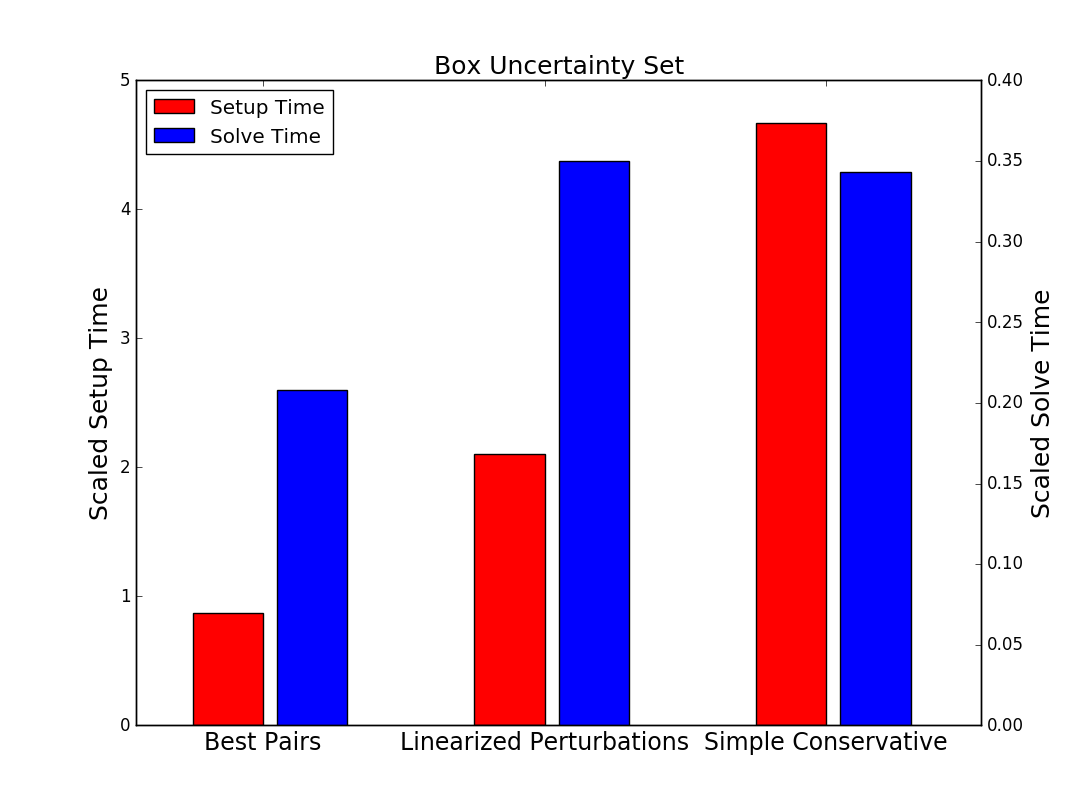
\includegraphics[height=2.3in]{signomial_simple_flight/box_times.png}
    \end{subfigure}
    ~
    \begin{subfigure}{0.49\textwidth}
        \centering
        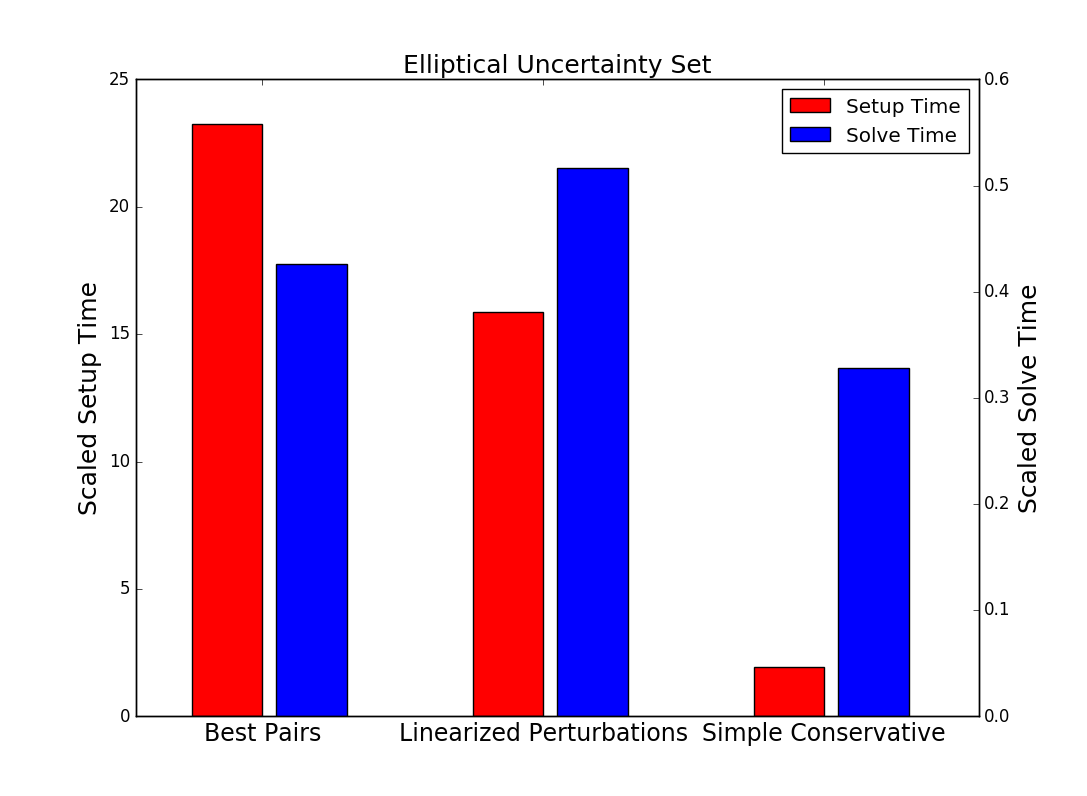
\includegraphics[height=2.3in]{signomial_simple_flight/ell_times.png}
    \end{subfigure}
    \caption{Robust signomial simple aircraft solution and setup times, normalized by the
    nominal problem solution time. Note that the problems with box uncertainty have much lower setup
    time costs versus those with elliptical uncertainty.}
    \label{compare_signomial}
\end{figure}

\subsection{The Effect of Robustness on Multiobjective Performance}

One of the benefits of convex and difference-of-convex optimization methods is the ability to optimize for
different objectives~\cite{York2018}. As a demonstration, we optimized the aircraft without uncertainty
for 7 different objectives, and show
the non-dimensionalized results in Table~\ref{tab:nondimresults}.

\begin{table}
    \resizebox{\textwidth}{!}{
    \csvautobooktabularcenter{figures/objective_table.csv}
    }
\caption{Non-dimensionalized variations in objective values with respect to the aircraft optimized
for different objectives. Objective values were normalized by the total fuel solution.}
    \label{tab:nondimresults}
\end{table}

Since the model is physics based, it is able to accommodate a range of objectives,
even ones that are not often considered such as aspect ratio. The resulting aircraft
also differ drastically with respect to performance and design variables.
As the most extreme example,
the aircraft optimized for time cost has 150 times the engine weight as the aircraft
optimized for total fuel, since a huge amount of power is required to fly fast.

Aside from this caricature example, we further demonstrate the capabilities of \gls{rsp}s in
multiobjective design by considering a more realistic scenario.
We perform the optimization of the aircraft with no uncertainty and ellipsoidal uncertainty ($\Gamma = 1$)
for 4 different objective functions, and plot the results on spider plots.
Spider plots are useful because they allow engineers to see the performance of
different designs in a multi-objective
environment. One way to envision the multi-objective
performance of the aircraft is to consider the area contained within the web defined by the aircraft's
performance; the smaller the web area the better.
Due to the large disparities in the potential values of design variables depending
on objective as shown in Table~\ref{tab:nondimresults}, we chose to demonstrate this using four objective functions
that would be expected to have a high degree of correlation and therefore yield similar aircraft designs. These were
 total (time and fuel) cost, total fuel, takeoff weight and mid-cruise lift-over-drag (L/D).

\begin{figure}
    \begin{center}
    \begin{tikzpicture}
        \node[inner sep=0] (center) at (0,0)
        {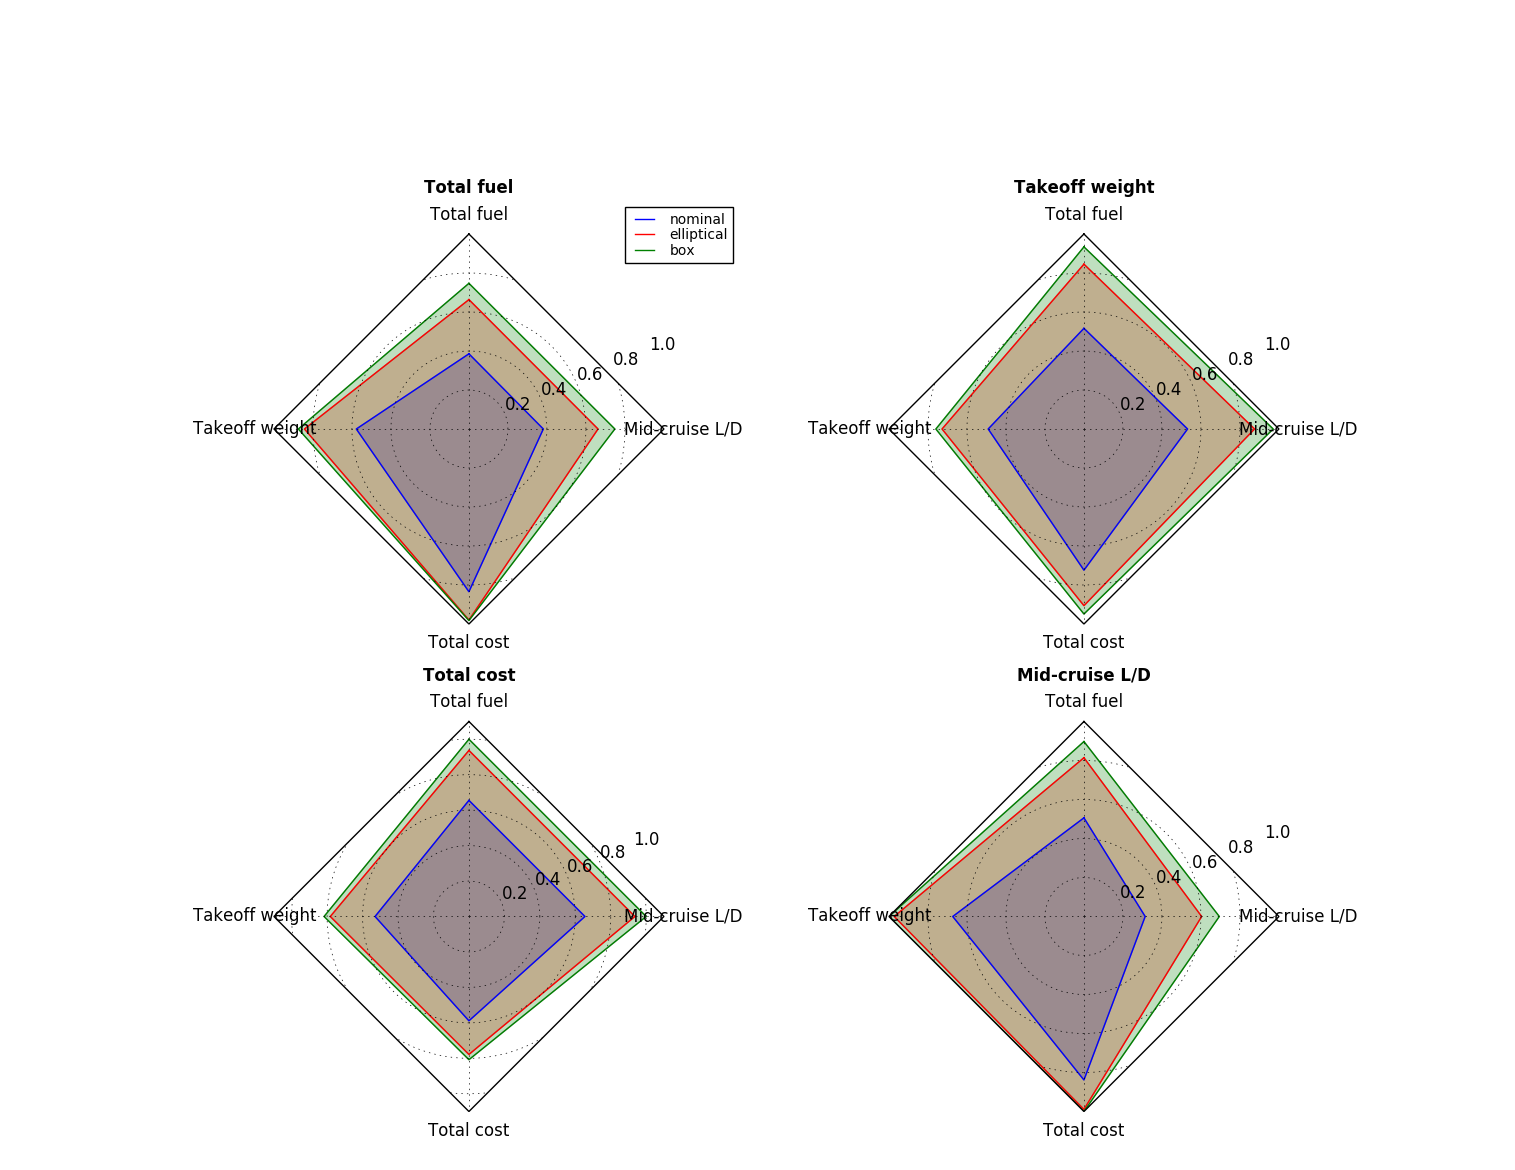
\includegraphics[trim={2cm 0 1cm 0},clip]{figures/4objradar.png}};
        \node[inner sep=0] (ur) at (0.68,0.25)
        {\includegraphics[trim={7cm 1cm 7cm 1cm}, clip, height=2.7cm]{figures/radar2.png}};
        \node[inner sep=0] (ll) at (-0.68,-2)
        {\includegraphics[trim={7cm 1cm 7cm 1cm}, clip, height=2.7cm]{figures/radar3.png}};
        \node[inner sep=0] (ul) at (-0.68, 0.25)
        {\includegraphics[trim={7cm 1cm 7cm 1cm}, clip, height=2.7cm]{figures/radar1.png}};
        \node[inner sep=0] (lr) at (0.68,-2)
        {\includegraphics[trim={7cm 1cm 7cm 1cm}, clip, height=2.7cm]{figures/radar4.png}};
    \end{tikzpicture}
    \caption{The spider plots of aircraft performance, for aircraft optimized for different objectives.
    The bolded titles are the design objectives for each plot, whereas the individual spiderwebs
    show the non-dimensionalized multiobjective performance of the aircraft designed under different
    uncertainty sets.}
    \label{fig:spider}
\end{center}
\end{figure}

\begin{figure}
    \begin{center}
        \begin{subfigure}{0.48\linewidth}
            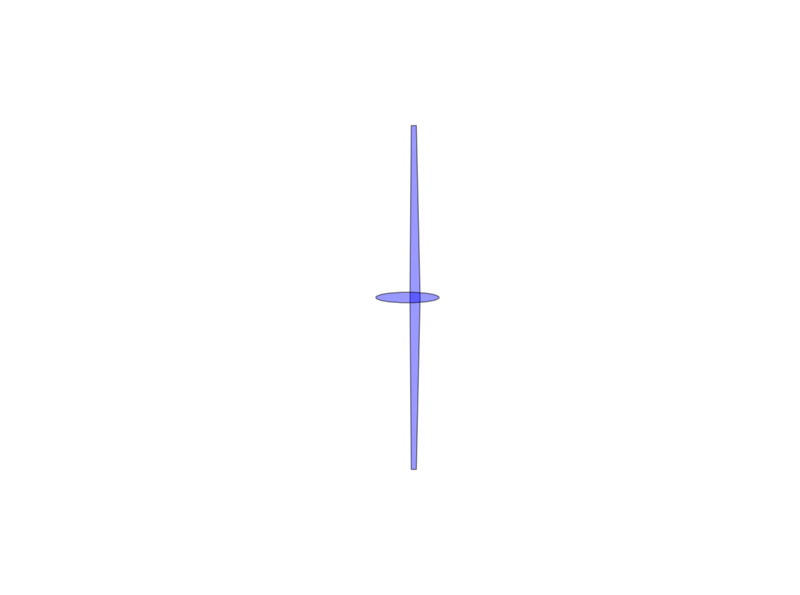
\includegraphics[trim={8cm 1cm 8cm 1cm}, clip, width=0.33\linewidth]{figures/0nominal.png}\hfill
            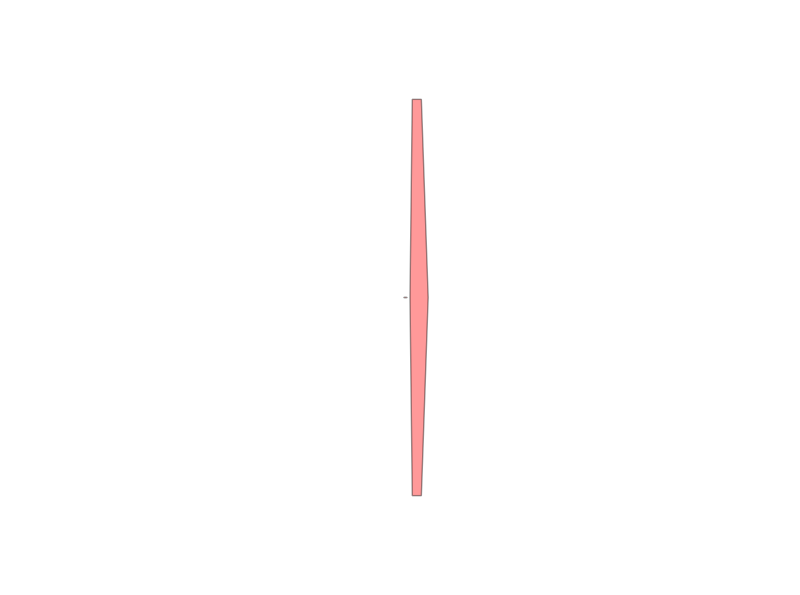
\includegraphics[trim={8cm 1cm 8cm 1cm}, clip, width=0.33\linewidth]{figures/0elliptical.png}\hfill
            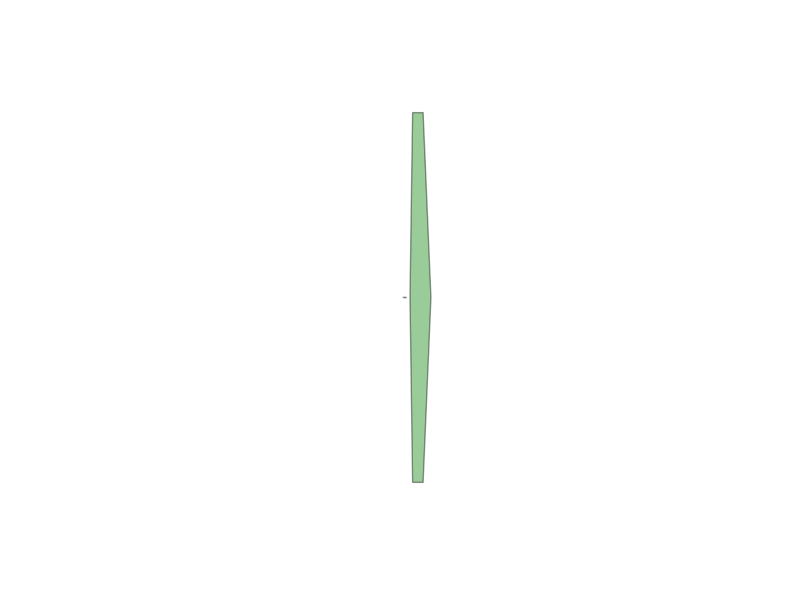
\includegraphics[trim={8cm 1cm 8cm 1cm}, clip, width=0.33\linewidth]{figures/0box.png}\hfill
            \caption{Total fuel}
        \end{subfigure}
        \begin{subfigure}{0.48\linewidth}
            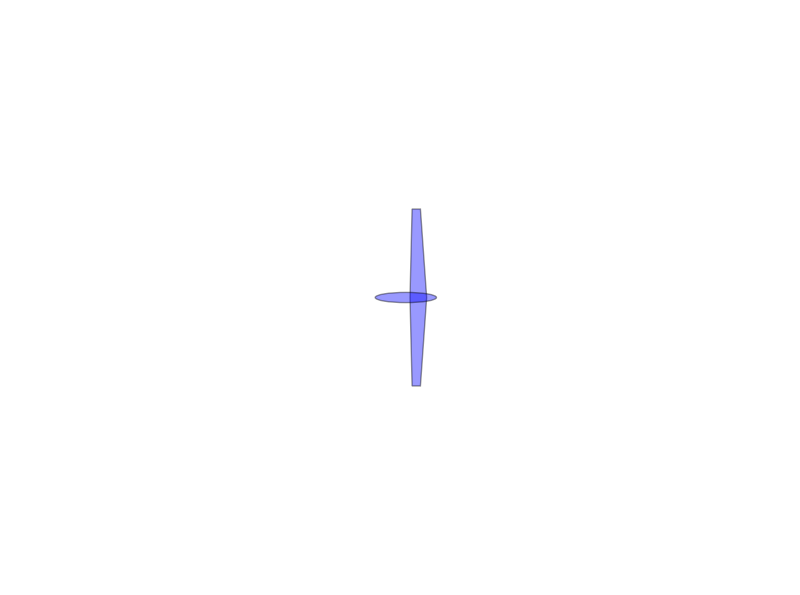
\includegraphics[trim={8cm 1cm 8cm 1cm}, clip, width=0.33\linewidth]{figures/1nominal.png}\hfill
            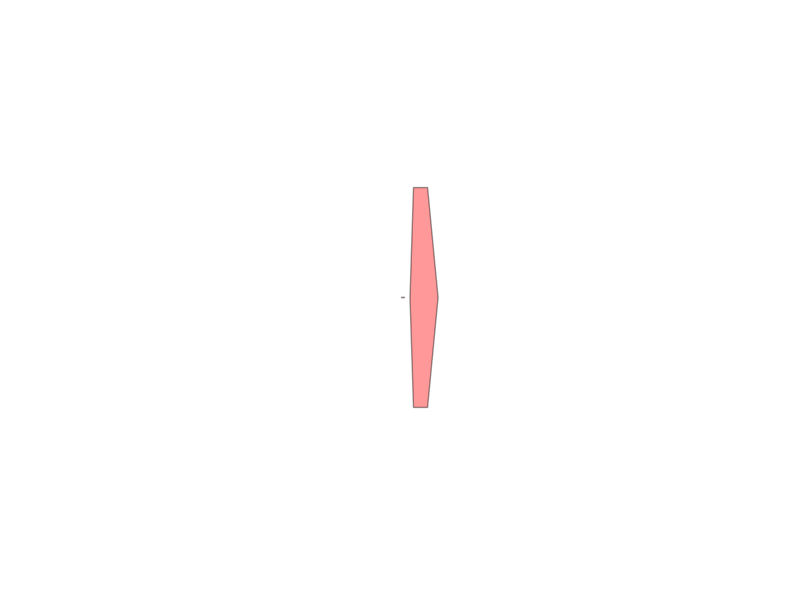
\includegraphics[trim={8cm 1cm 8cm 1cm}, clip, width=0.33\linewidth]{figures/1elliptical.png}\hfill
            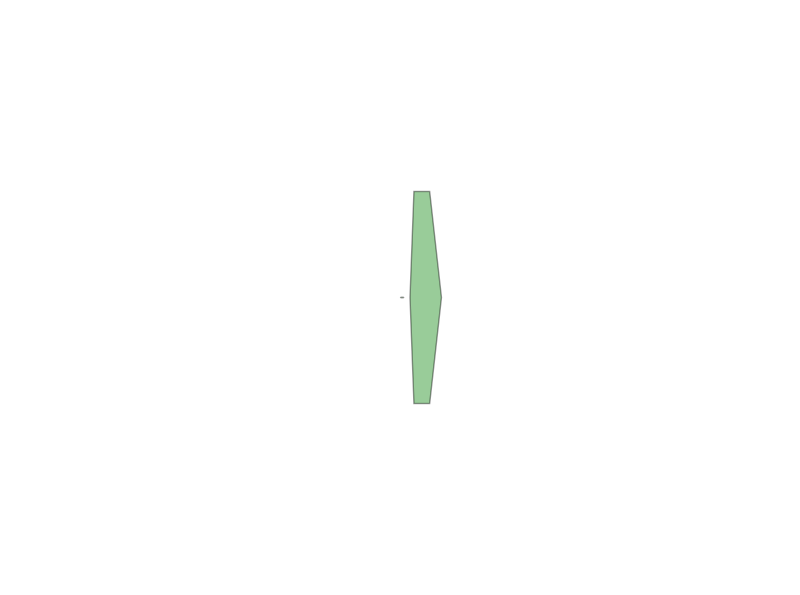
\includegraphics[trim={8cm 1cm 8cm 1cm}, clip, width=0.33\linewidth]{figures/1box.png}\hfill
            \caption{Takeoff weight}
        \end{subfigure}
        \begin{subfigure}{0.48\linewidth}
            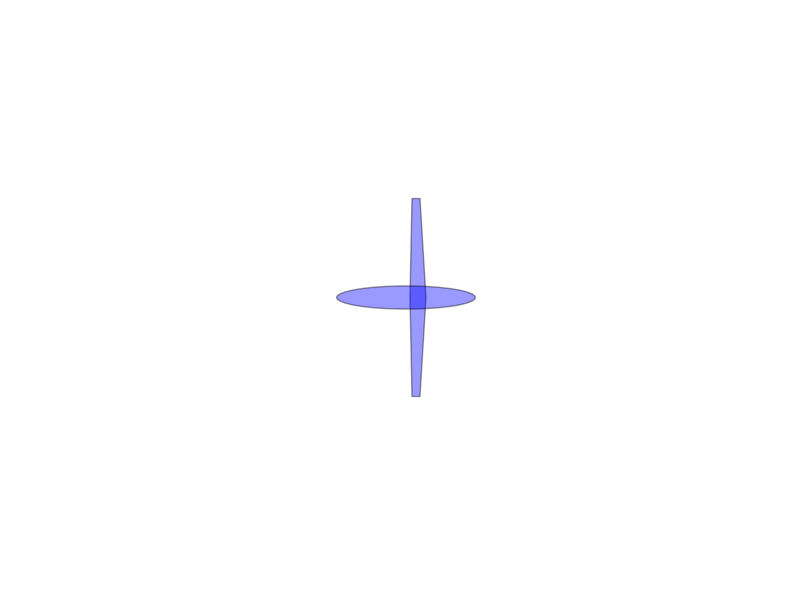
\includegraphics[trim={8cm 1cm 8cm 1cm}, clip, width=0.33\linewidth]{figures/2nominal.png}\hfill
            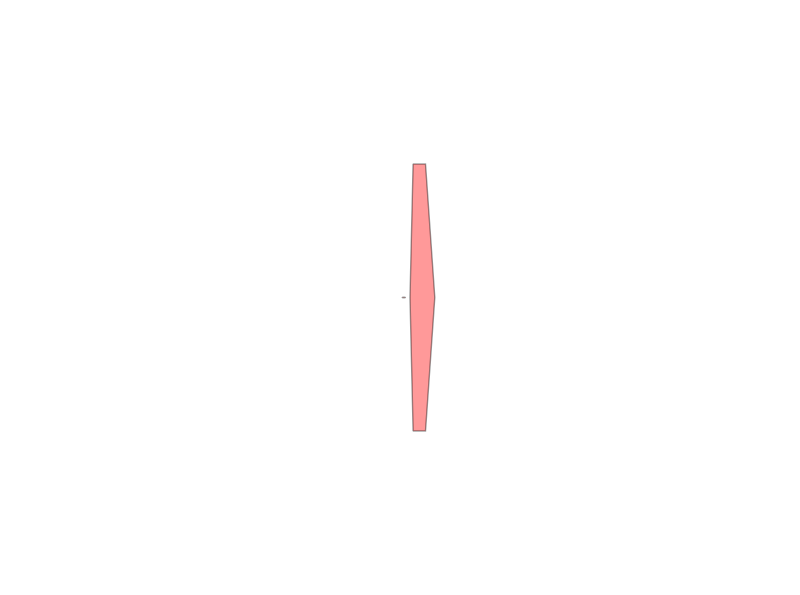
\includegraphics[trim={8cm 1cm 8cm 1cm}, clip, width=0.33\linewidth]{figures/2elliptical.png}\hfill
            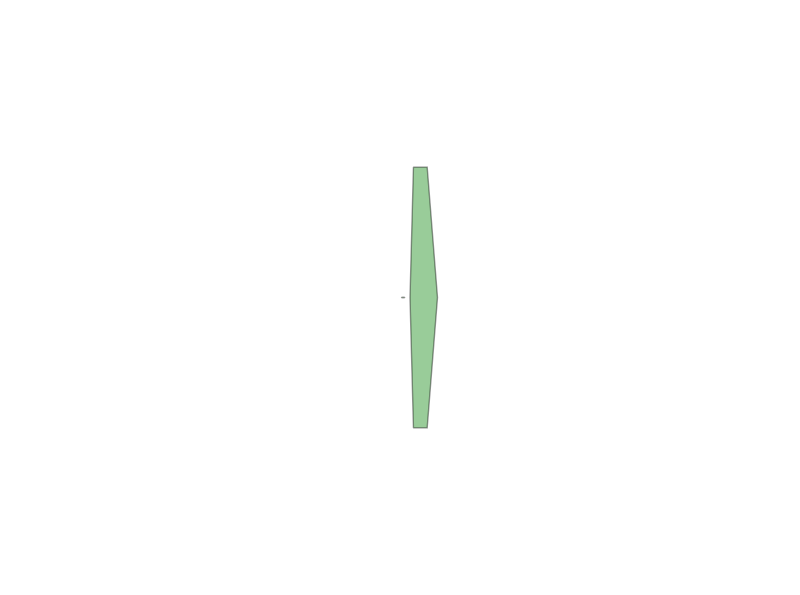
\includegraphics[trim={8cm 1cm 8cm 1cm}, clip, width=0.33\linewidth]{figures/2box.png}\hfill
            \caption{Total cost}
        \end{subfigure}
        \begin{subfigure}{0.48\linewidth}
            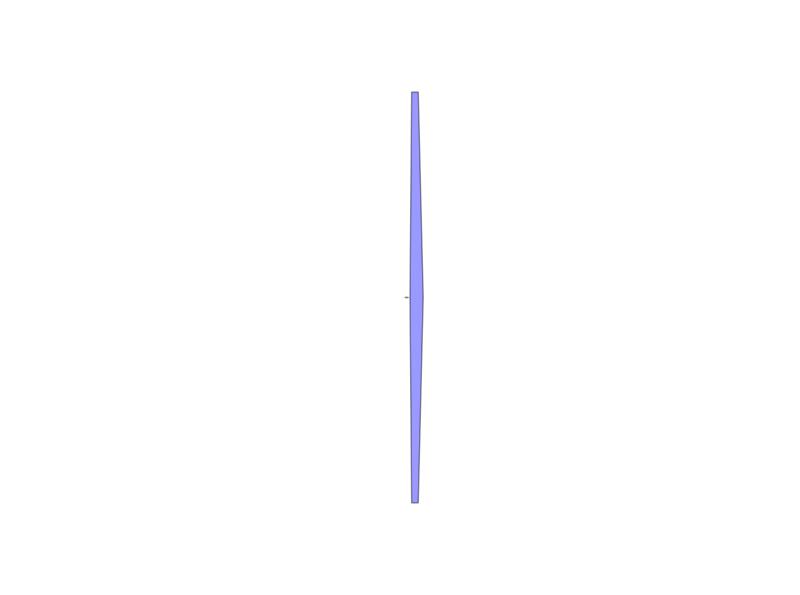
\includegraphics[trim={8cm 1cm 8cm 1cm}, clip, width=0.33\linewidth]{figures/3nominal.png}\hfill
            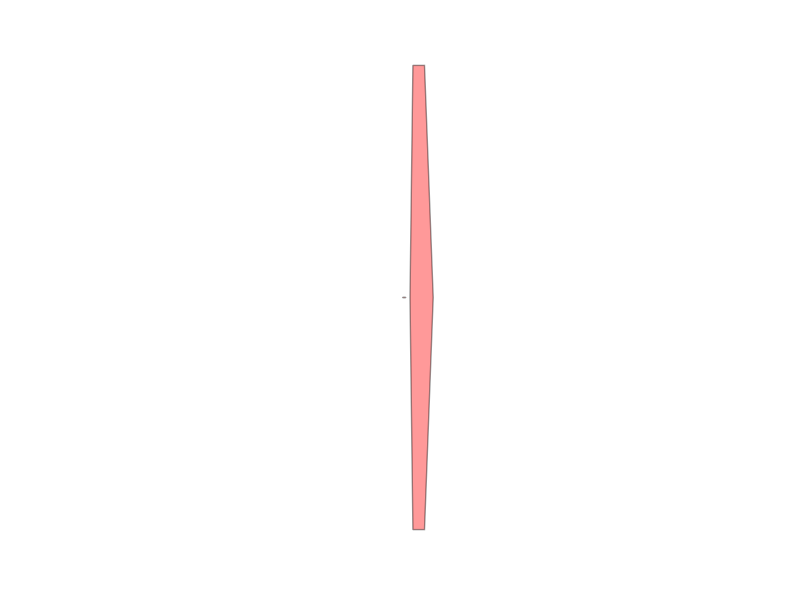
\includegraphics[trim={8cm 1cm 8cm 1cm}, clip, width=0.33\linewidth]{figures/3elliptical.png}\hfill
            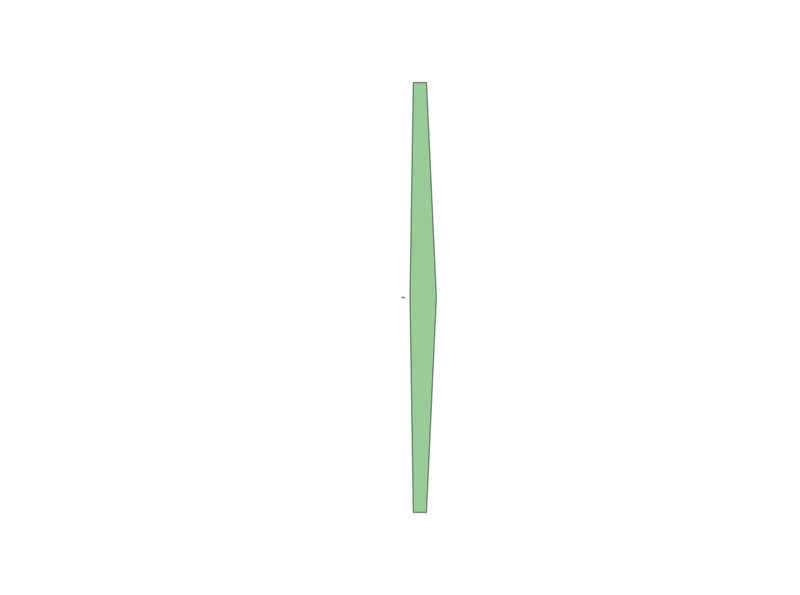
\includegraphics[trim={8cm 1cm 8cm 1cm}, clip, width=0.33\linewidth]{figures/3box.png}\hfill
            \caption{Mid-cruise L/D}
        \end{subfigure}\par\medskip
        \caption{Sketches of the aircraft drawn for corresponding spider plots. Drawn to scale for comparison.}
    \end{center}
\end{figure}

In the spider plots in Figure~\ref{fig:spider}, it is possible to see the effect of robustness on
the different worst-case performance metrics of the different aircraft. In this example, four objectives that
are highly coupled were chosen to make sure the we can do a comparative graphical analysis.
For the nominal case, it is possible to see that
the aircraft designed for total fuel performs the best when all four objectives are considered,
assuming that all objectives are weighted equally. As expected,
the box uncertainty set is strictly more conservative than the elliptical uncertainty set, for
all objectives. In this case, it is true that total fuel is the objective that maximizes
the multiobjective outcome, but for certain \gls{rsp}s it is possible that the multiobjective behavior
of aircraft designed using different uncertainty sets

And interestingly enough, there is a convergence in the geometry of the aircraft as they are designed
to be robust to uncertain outcomes. All of the robust designs eschew the storage of fuel in the fuselage
for larger wings that can store more fuel. This is not to say that none of the aircraft will ever have
fuselages; one example is a mission where flight time is a much more important objective
than fuel weight.

% TODO: add robust cases where there is a fuselage.


In absence of understanding of the role of uncertainty in aircraft design,

TODO: flesh out.
This analysis could also be performed for the mean performance
of the aircraft determined through ~\gls{mc} simulation, but this demonstration limits
its scope to the worst-case analysis.

\subsection{Risk minimization problems}

All of the previous multi-objective analyses have assumed that we have an
understanding of exactly how much risk we are
willing to tolerate. However, it would also make sense if risk was the objective of our
model. This would suggest the following formulation:

\begin{align*}
    \text{max} &~\Gamma \\
    \text{s.t.}     &~f_i(x,u) \leq 0, i = 1,\ldots,n \\
                    & \norm{u} \leq \Gamma \\
                    &~f_0(x) \leq (1+\delta)f_0^*,~\delta \geq 0 \tag{a}
    \label{eq:goalprogramming}
\end{align*}

where $f_0^*$ is the optimum of the nominal problem in Formulation~\ref{eq:normform}, $\delta$
is a fractional measure of the objective that we are willing to sacrifice for robustness, which
gives $(1+\delta)f_0^*$ as the upper bound on the objective value. Intuitively,
this is a form of goal programming,
where we specify the exact maximum worst-case value of an objective we can tolerate so that the program
risk is acceptable, but in the meanwhile maximize the total size of the uncertainty we can handle.
We call the method of minimizing an objective for set ${\Gamma}$ \emph{the $\Gamma$ method},
while we call the goal programming approach, which maximizes $\Gamma$ for a set $\delta$,
\emph{the $\delta$ method}.

The problem in Formulation~\ref{eq:goalprogramming} is not equivalent to the problem in Formulation~\ref{eq:normform},
but should yield the same result. As a proof of concept, we perform the same probability of failure
analysis as in Figure~\ref{fig:deltaVsGamma}, but have the objective bound be an input to the
optimization problem and the $\Gamma$ of the uncertainty set be maximized.

\begin{figure}[ht]
    \centering
    \captionsetup{justification=centering, font=small}
    \begin{subfigure}{0.49\textwidth}
        \centering
        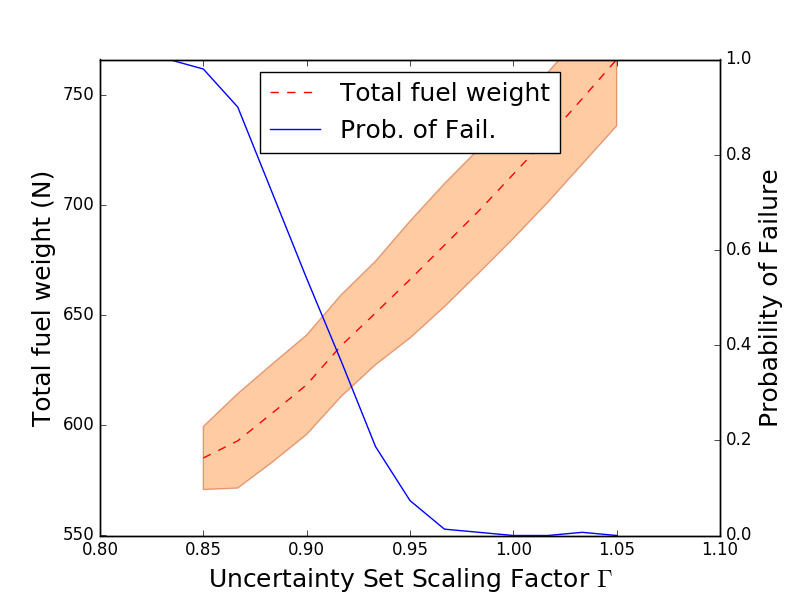
\includegraphics[height=2.3in]{signomial_simple_flight/ell_best_pairs.png}
         \caption{Elliptical Uncertainty, $\Gamma$ method}
    \end{subfigure}%
    ~
    \begin{subfigure}{0.49\textwidth}
        \centering
        \includegraphics[height=2.3in]{signomial_simple_flight/deltaResults.png}
         \caption{Elliptical Uncertainty, $\delta$ method}
    \end{subfigure}
    \caption{Simulated performance of the optimal robust aircraft, using the Best Pairs formulation
    for the $\Gamma$ and $\delta$ methods.
    The dashed line and the band represent the mean and standard deviation of the performance
    of aircraft designed for different $\Gamma$,
    and simulated with 100 \gls{mc} samples of uncertain parameters.}
    \label{fig:deltaVsGamma}
\end{figure}

As expected, we get identical results from the outputs of the two formulations (to confirm).
We can also expand this framework to perform multivariate goal programming,
by changing (a) in the formulation~\ref{eq:goalprogramming} to include all
objectives we are interested in.

\begin{align*}
    f_{0,j}(x) \leq (1+\delta_j) f^*_{0,j},~\delta_j \geq 0,~j = 1,\ldots, m
    \label{eq:multigoal}
\end{align*}

The benefit of goal programming is that it allows us to explore multidisciplinary tradeoffs without
having to enumerate the design space along each objective direction.
In design it is not obvious whether an objective should in fact be a constraint instead. The most
fundamental choice that an engineer can make in design is what the objective function is, and it is
often the case that there are many potential objectives that are conflicting. The term multiobjective optimization is misleading
because you can only optimize for one objective at once,
and the design is going to be influenced by how engineers weight different objectives.
Risk minimization makes these implicit decisions explicit, empowers engineers to choose
how much performance they would be willing to sacrifice with respect
to optimal but fragile designs to obtain robust designs, and gives a prediction of the margin of error
for every parameter that they have to make designs feasible.

\section{Potential Future Work or Studies}

There are a myriad of potential extensions to signomial programming under uncertainty.
In the spirit of helping reduce program risk in aerospace design,
the authors make a few observations and recommendations.

In this study, we do not discriminate between the kinds of constraints violated. However, it would
be possible to rank the severity of constraint violations so as to penalize some (eg. structural safety)
more heavily than others (maximum range constraint). This would inject further realism into the
design under uncertainty since some violations contribute to program risk more
strongly than others.

Another potentially valuable extension to the proposed framework is the concurrent implementation
of multiple sets to contain the uncertain parameters, with the purpose of restricting uncertain
outcomes further. One example of this would be to impose an  L1-norm on the integer number of uncertain parameters
as well as an L2-norm on the overall size of uncertainty set
This method can be used to set the total size of the uncertainty set in a Euclidian sense,
but then also to restrict the stochasticity to a subset of all of the uncertain parameters,
thereby somewhat restricting nature. This also turns the problem into an integer robust
optimization problem which poses interesting computational challenges.

With respect to interesting studies, \gls{ro} opens up many possibilities to discover and analyze the benefits
of adaptable architectures in aircraft design versus more traditional point designs
when faced with parametric uncertainty. Some examples of these are modular designs, morphing designs,
adaptively manufactured designs and aircraft families. It is likely that these types of engineered
robustness become more effective at reducing program risk in presence of uncertainty, since they are more likely
to deliver value under adverse stochastic outcomes.

In situations where there is data available to aid design, \gls{ro} can help explore
the design space while taking into account the stochasticity and noise in the data.
This opens up an array of potential trade studies where engineers can learn about
the exposure of designs to the sparsity and spread of data and attempt to gather
data which best reduces the uncertainty in the performance of optimal designs.


\section{Conclusion}

This paper has motivated the use of robust optimization in conceptual engineering
design, in lieu of the mathematically non-rigorous methods of optimization under uncertainty
widely used in the aerospace industry today. We have developed a tractable \gls{rsp} formulation
in response to a need to optimize over uncertain parameters, extending
the tractable approximate RGP framework developed by Saab~\cite{Saab2018} to non-log-convex problems.
This \gls{rsp} formulation is a valuable contribution to the fields of robust
optimization and difference-of-convex programming.

\gls{rsp}s have a wide variety of potential applications in engineering design.
We demonstrated using a simple aircraft design problem
that using \gls{ro}, and specifically \gls{rsp}s in conceptual aircraft design will result in systems
that are more robust with respect to uncertainties in operational parameters,
such as payload mass and range, as well as uncertain environmental and manufacturing parameters.
Unlike legacy methods, this robustness has probabilistic guarantees, where sets of size $\Gamma=1$
protect against all realizations of uncertainty for a given set of parameters.
Thus engineers can use robust signomial programming to trade off
robustness and optimality within engineered systems in a tractable and mathematically rigorous manner.

We compared the results of designs created using box and elliptical uncertainty sets, where the
box uncertainty approximates the use of margins in design. We
confirmed that designs using elliptical uncertainty are strictly less conservative
than those that would be generated through the use of box uncertainty while protecting against the same
parametric uncertainties. Since designs found using robust signomial programming
under elliptical uncertainty are less conservative
than designs found through traditional methods, \gls{rsp}s have the potential to reduce
the program risk and increase the performance
of designs compared to traditional methods with no sacrifice in reliability.

\gls{ro} has the potential to change current aerospace design paradigms by introducing
mathematical rigor to design under uncertainty. Current aerospace
conceptual design practices still rely heavily on the expertise of established
engineers even in absence of prior experience exploring the design space.
\gls{rsp}s provide new opportunities in aerospace conceptual design
since they are compatible with physics based models
that are deprived of or lacking in data, and bring quantitative
measures of design reliability to the table.


\section*{Appendix}

\subsection{Robust Linear Programming: A Quick Review} \label{LP_to_GP}

As mentioned earlier, principles from robust linear programming are used
formulate an approximate robust geometric program.\\[12pt]
Consider the system of linear constraints
\begin{equation*}
    \mathbb{A}\mathbf{x} + \mathbf{b} \leq 0
\end{equation*}
where
\begin{align*}
    \mathbb{A} &\text{ is $m \times n$}\\
    \mathbf{x} &\text{ is $n \times 1$}\\
    \mathbf{b} &\text{ is $m \times 1$}\\
\end{align*}
where the uncertain data is contained in a set defined by equations \eqref{Data} and \eqref{perturbation_set}.

\subsubsection{Box Uncertainty Set}
If the perturbation set $\mathcal{Z}$ given in equation \eqref{perturbation_set} is a box
uncertainty set, i.e. $\|\mathbf{\zeta}\|_{\infty} \leq \Gamma$, then the robust formulation of the $i$th constraint is equivalent to
\begin{equation}
    \Gamma \textstyle{\sum}_{l=1}^L |- {b}^l_{i} - \mathbf{a}^l_i\mathbf{x}| + \mathbf{a}^0_i\mathbf{x} + b^0_i \leq 0
    \label{box_absolute}
\end{equation}
If only $b$ is uncertain, i.e. $A^l = 0,~\forall l = 1,2,...,L$, then equation \eqref{box_absolute} becomes
\begin{equation}
    \textstyle{\sum}_{l=1}^L \mathbf{a}^0_{i}\mathbf{x} + b^0_{i} + \Gamma \textstyle{\sum}_{l=1}^L |b^l_{i}| \leq 0
    \label{box_coeff}
\end{equation}
which is a linear constraint.

On the other hand, if $A$ is uncertain, the equation \eqref{box_absolute} is equivalent to the following set of linear constraints
\begin{equation}
    \label{box_linear}
    \begin{split}
        \Gamma \textstyle{\sum}_{l=1}^L w^l_{i} + \mathbf{a}^0_{i}\mathbf{x} + b^0_{i} &\leq 0 \\
        - b^l_{i} - \mathbf{a}^l_{i}\mathbf{x} &\leq w^l_{i},~\forall l \in 1,...,L\\
        b^l_{i} + \mathbf{a}^l_{i}\mathbf{x} &\leq w^l_{i},~\forall l \in 1,...,L\\
    \end{split}
\end{equation}

\subsubsection{Elliptical Uncertainty Set}
If the perturbation set $\mathcal{Z}$ is an elliptical, i.e. $\textstyle{\sum}_{l=1}^L\frac{\zeta_l^2}{\sigma_l^2} \leq \Gamma^2$,
then the robust formulation of the $i^{th}$ constraint is equivalent to
\begin{equation}
    \Gamma \sqrt{\textstyle{\sum}_{l=1}^L \sigma_l^2(- b^l_{i} - \mathbf{a}^l_{i}\mathbf{x})^2} + \mathbf{a}^0_{i}\mathbf{x} + b^0_{i} \leq 0
    \label{ell_absolute}
\end{equation}
which is a second order conic constraint.

If only $b$ is uncertain, i.e. $\mathbb{A}^l = 0,~\forall l = 1,2,...,L$, then equation \eqref{ell_absolute} becomes
\begin{equation}
    \textstyle{\sum}_{l=1}^L \mathbf{a}^0_{i}\mathbf{x} + b^0_{i} + \Gamma \sqrt{\textstyle{\sum}_{l=1}^L \sigma_l^2(b^l_{i})^2} \leq 0
    \label{ell_coeff}
\end{equation}
which is a linear constraint.

\subsubsection{Norm-1 Uncertainty Sets}

If the perturbation set represented by $\mathcal{Z}$ is a norm-1 uncertainty set, i.e. $\|\mathbf{\zeta}\|_1 \leq \Gamma$,
then the robust constraint is
\begin{equation}
    \textstyle{\sum}_{l=1}^L \mathbf{a}^0_{i}\mathbf{x} + b^0_{i} + \Gamma \max_{l=1,..,L} |b^l_{i}| \leq 0
    \label{rom_coeff}
\end{equation}
when $\mathbb{A}^l = 0$, and
\begin{equation}
    \begin{split}
        \Gamma w_{i} + \mathbf{a}^0_{i}\mathbf{x} + b^0_{i} &\leq 0 \\
        - b^l_{i} - \mathbf{a}^l_{i}\mathbf{x} &\leq w_{i},~\forall l \in 1,...,L\\
        b^l_{i} + \mathbf{a}^l_{i}\mathbf{x} &\leq w_{i},~\forall l \in 1,...,L\\
    \end{split}
    \label{rom_linear}
\end{equation}
if $\mathbb{A}^l \neq 0$. Note that for this type of uncertainty, the robust constraints are linear.


\section*{Acknowledgments}

A place to recognize others.

\bibliographystyle{aiaa}
\bibliography{main}

\end{document}

% - Release $Name:  $ -
